\chapter{内在的幾何学とテンソルの代数}

テンソル記法は、それが思考の一部を代行してくれるときにのみ有用である。よく設計された記法は機械部品の箱のように振る舞う。上付き添字は下付き添字と噛み合い、異なる種類の対象どうしは加えられることを拒み、合法な縮約は、残った添字からその変換則が読み取れるような対象を残す。この仕組みの当面の目的は幾何学的なものである。われわれは、真の曲率と、座標が曲げられたためにのみ現れる曲率とを区別したいのである。

\section{内側から見た曲率}

まず普通の一枚の紙から始めよう。それは引き伸ばしたり破いたりすることなく円筒に丸めることができる。周囲の部屋にいる観測者にとって、その紙は明らかに曲がっている。それにもかかわらず、紙の内部で測られる距離は変わらない。その外的曲率は変化したが、内在的幾何学は変化していないのである。

次に、その紙に閉じ込められた小さな生き物を想像しよう。それは周囲の部屋を覗くことができない。長さを測り、隣り合う方向を比較し、三角形を構成し、測定棒を場所から場所へ運ぶことができる。それらの内部的な実験こそが、幾何学に要求されるべきすべてである。重力における対応する問いは、ある場が真の時空の曲率を表しているのか、それとも平坦な時空の単なる曲線的な記述にすぎないのか、ということである。

この内在的な視点を具体的にする一つの方法は、曲面を点と連結のネットワークで置き換えることである。隣り合う点を結び、すべての連結の長さを記録し、関節が蝶番のように動くことを許す。正三角形の格子は平坦に横たわる。関節を曲げても、符号化された幾何学は変わらない。なぜなら、格子は長さを一つも変えることなく常に平面に戻すことができるからである。

次に、一つの頂点で交わる六本の連結を、周囲の連結を固定したまま長くしよう。中心の頂点は、定められた長さを破ることなく平面内にとどまることがもはやできない。それは盛り上がって膨らみとならなければならない。この曲率を診断するのに外からの眺めは必要なかった。両立しない隣接距離がすでにそれを含んでいたのである。

\begin{figure}[H]
\centering
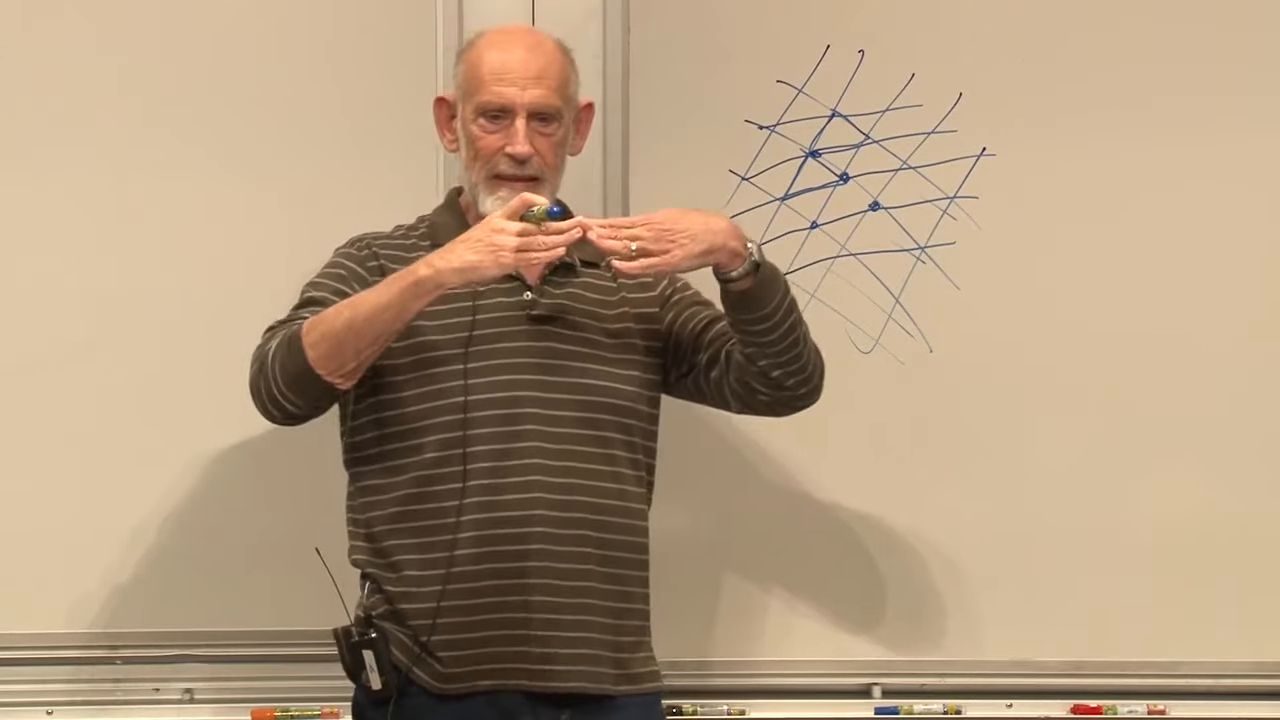
\includegraphics[width=\linewidth]{lecture_02_figure_01.png}
\caption{内在的幾何学の三角形連結模型。一つの頂点の周りの連結を変えると、長さを変えずには平坦化できない膨らみが強制される。}
\lectureframe{00:06:40}
\end{figure}

\begin{classroomqa}
\audiencequestion{では、平坦な空間の正確な定義とは何か。}
\lecturerresponse{操作的な答えは、その内在的な距離関係がユークリッド的な配置において歪みなく実現できることである。以下で展開する言葉で言えば、リーマン空間は、関心のある領域全体にわたって計量が定数クロネッカーのデルタとなるような座標を見つけることができるとき、平坦である。一つの点においてはこれは常に局所的に行うことができる。それを一つの領域にわたって行うことが非自明な条件である。曲率テンソルは、最終的に、特別な座標の選択に言及することなくその条件を述べることになる。
\lecturetimestamp{00:09:15}}
\end{classroomqa}

この答えは、われわれがまだ獲得していない計量を用いている。したがってわれわれは一時的に曲率からテンソル解析へと向きを変える。この寄り道は任意ではない。計量の座標依存性を真の幾何学から分離する前に、計量がテンソルであると認識されなければならないのである。

\section{場と座標による記述}

一般相対性理論におけるテンソルは、通常はテンソル\emph{場}である。すなわち、各点にテンソルがあり、その成分は点ごとに変化する。スカラー場は最も単純な例である。曲面上の温度は、各点\(P\)における数\(S(P)\)によって表すことができる。二人の人がその点を異なる座標でラベル付けしても、そこの温度については一致しなければならない。

\begin{figure}[H]
\centering
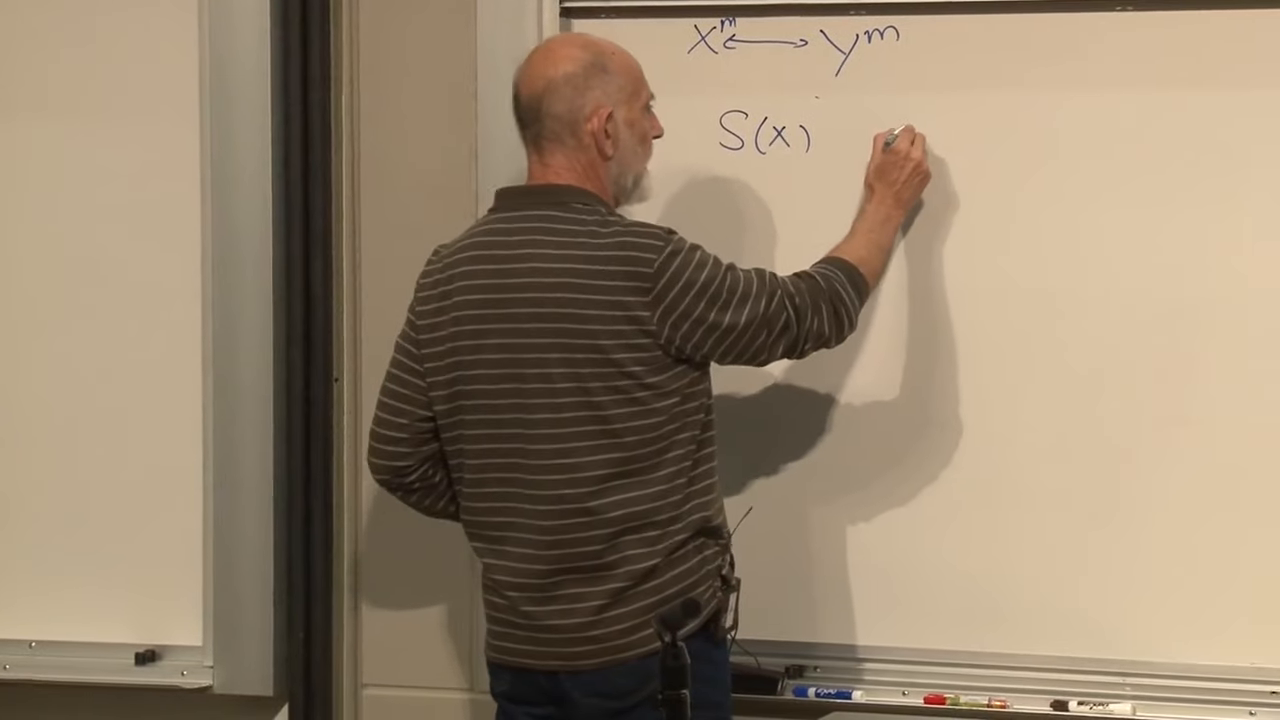
\includegraphics[width=\linewidth]{lecture_02_figure_02.png}
\caption{スカラー場と、同じ点に対する二つの座標ラベル。}
\lectureframe{00:11:25}
\end{figure}

\(x^m\)と\(y^m\)を二つの滑らかな座標系とする。それぞれは点から数の順序付けられたリストへの写像であり、重なり合う座標パッチにおいて、二つのリストは互いに逆の関数によって関係づけられる。
\begin{equation}
 y^m=y^m(x^1,\ldots,x^d),
 \qquad
 x^m=x^m(y^1,\ldots,y^d).
\label{eq:coordinate-maps}
\end{equation}
滑らかさは微分を可能にし、可逆性は、座標を変えるだけで点が失われたり別の点と同一視されたりしないことを保証する。

\begin{figure}[H]
\centering
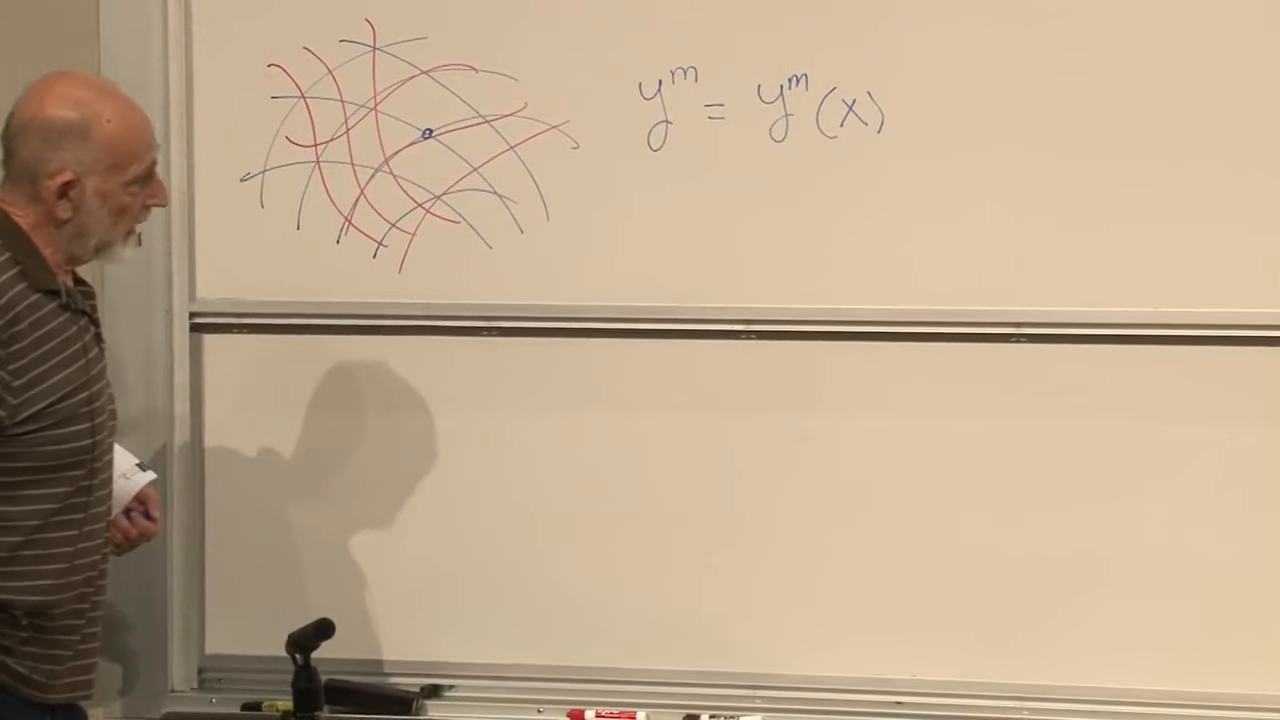
\includegraphics[width=\linewidth]{lecture_02_figure_03.png}
\caption{同じ幾何学的領域を記述する二つの滑らかで可逆な座標写像。}
\lectureframe{00:13:10}
\end{figure}

スカラー場に対して、変換則は単に
\begin{equation}
 S'(y)=S(x).
\label{eq:scalar-law}
\end{equation}
である。両辺の関数は、その引数が異なるために異なって見えるかもしれないが、対応する点においてそれらの値は一致する。これは不変な言明の原型である。

\section{斜交座標と二種類の成分}

一般的なテンソルを変換則によって定義する前に、上付きと下付きのベクトル添字がなぜ互いの装飾的な変種として扱えないのかを見ておくことは有用である。

軸が直交しておらず、規格化もされていない座標格子を描く。ある点において、\(x^m\) を1座標単位だけ増やすと、基底ベクトル \(\mathbf e_m\) が生じる。座標の言葉では、
\begin{equation}
 \mathbf e_m=\frac{\partial \mathbf r}{\partial x^m}.
\label{eq:coordinate-basis}
\end{equation}
ベクトル \(\mathbf e_m\) は単位長である必要はなく、直交している必要もない。

\begin{figure}[H]
\centering
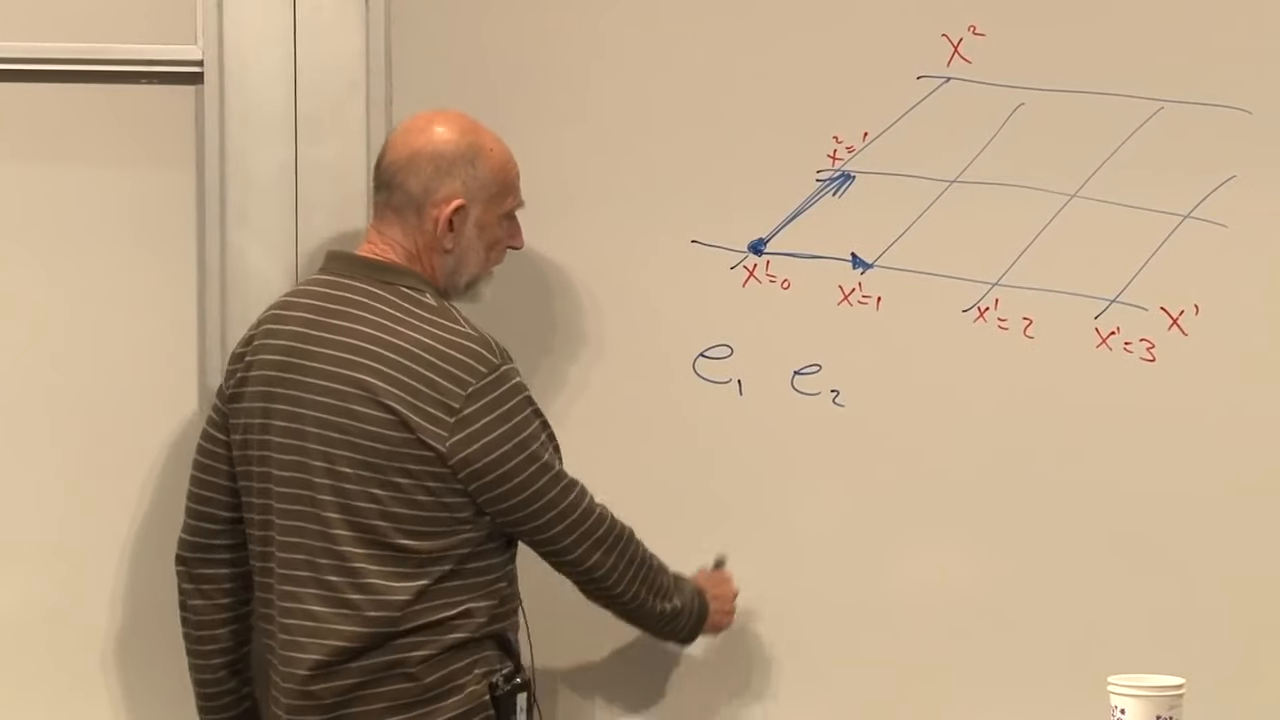
\includegraphics[width=\linewidth]{lecture_02_figure_04.png}
\caption{斜交座標格子とその座標基底ベクトル。}
\lectureframe{00:17:40}
\end{figure}

任意のベクトル \(\mathbf V\) はこの基底で展開できる：
\begin{equation}
 \mathbf V=V^m\mathbf e_m.
\label{eq:contravariant-expansion}
\end{equation}
数 \(V^m\) は \emph{反変成分} である。それらは、基底ベクトルから幾何学的ベクトルを組み立てるのに必要な係数である。

\begin{figure}[H]
\centering
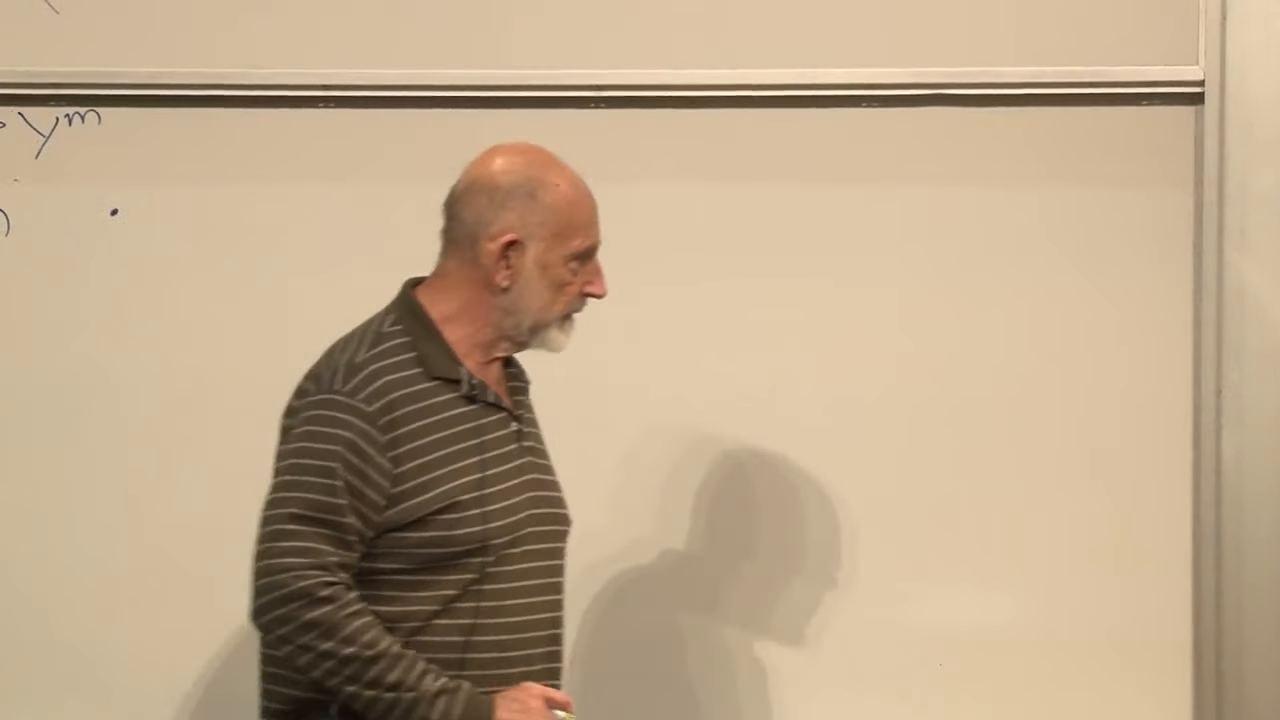
\includegraphics[width=\linewidth]{lecture_02_figure_05.png}
\caption{非直交座標基底におけるベクトルの展開。}
\lectureframe{00:19:20}
\end{figure}

もう一組の自然な数の集合がある：
\begin{equation}
 V_m=\mathbf V\mathbin{\boldsymbol{\cdot}}\mathbf e_m.
\label{eq:covariant-projection}
\end{equation}
これらは \emph{共変成分} である。斜交基底では、それらは単に同じ係数の添字を動かしたものではない。\eqref{eq:contravariant-expansion} を代入すると
\begin{equation}
 V_m
 =V^n\bigl(\mathbf e_n\mathbin{\boldsymbol{\cdot}}\mathbf e_m\bigr).
\label{eq:covariant-from-basis}
\end{equation}

\begin{figure}[H]
\centering
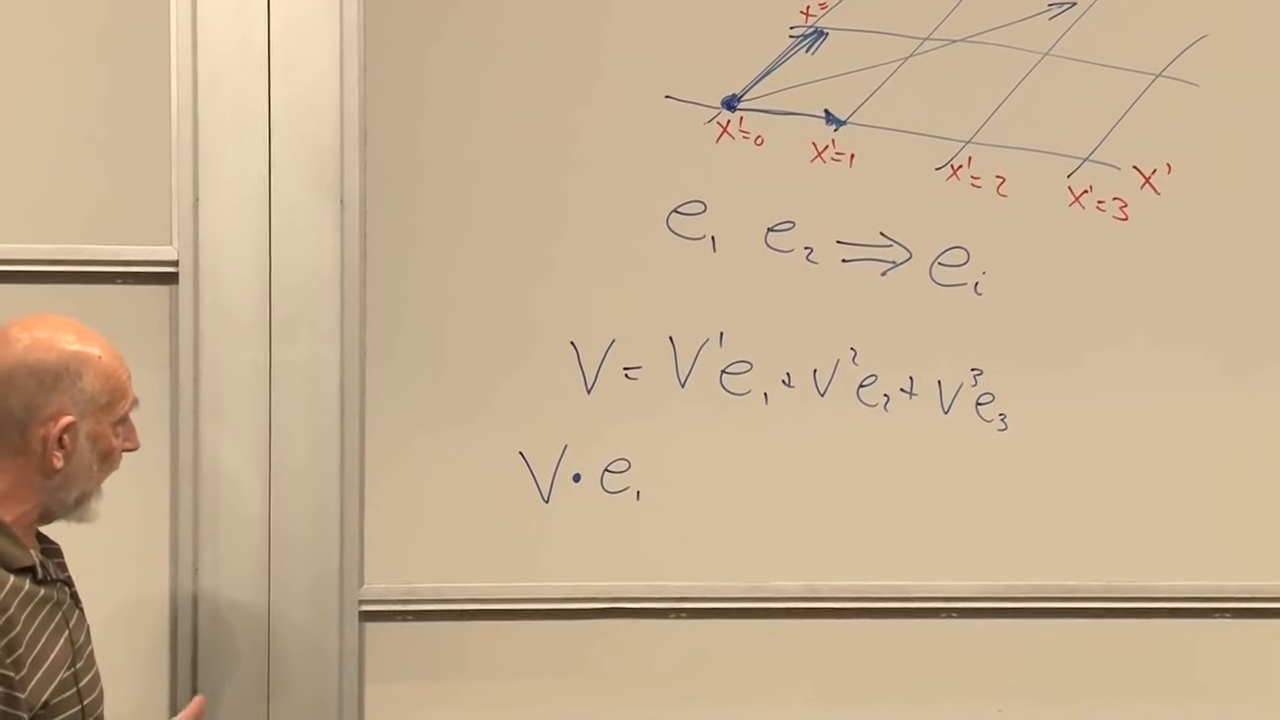
\includegraphics[width=\linewidth]{lecture_02_figure_06.png}
\caption{座標基底とのスカラー積をとることによって得られる共変成分。}
\lectureframe{00:21:10}
\end{figure}

基底ベクトルのスカラー積はグラム行列をなす：
\begin{equation}
 g_{mn}=\mathbf e_m\mathbin{\boldsymbol{\cdot}}\mathbf e_n.
\label{eq:metric-gram}
\end{equation}
したがって、
\begin{equation}
 V_m=g_{mn}V^n.
\label{eq:lower-vector}
\end{equation}
これが計量の最初の登場である。計量は座標基底の長さと相互の角度の両方を記録するため、展開係数を射影に変換する。

\begin{figure}[H]
\centering
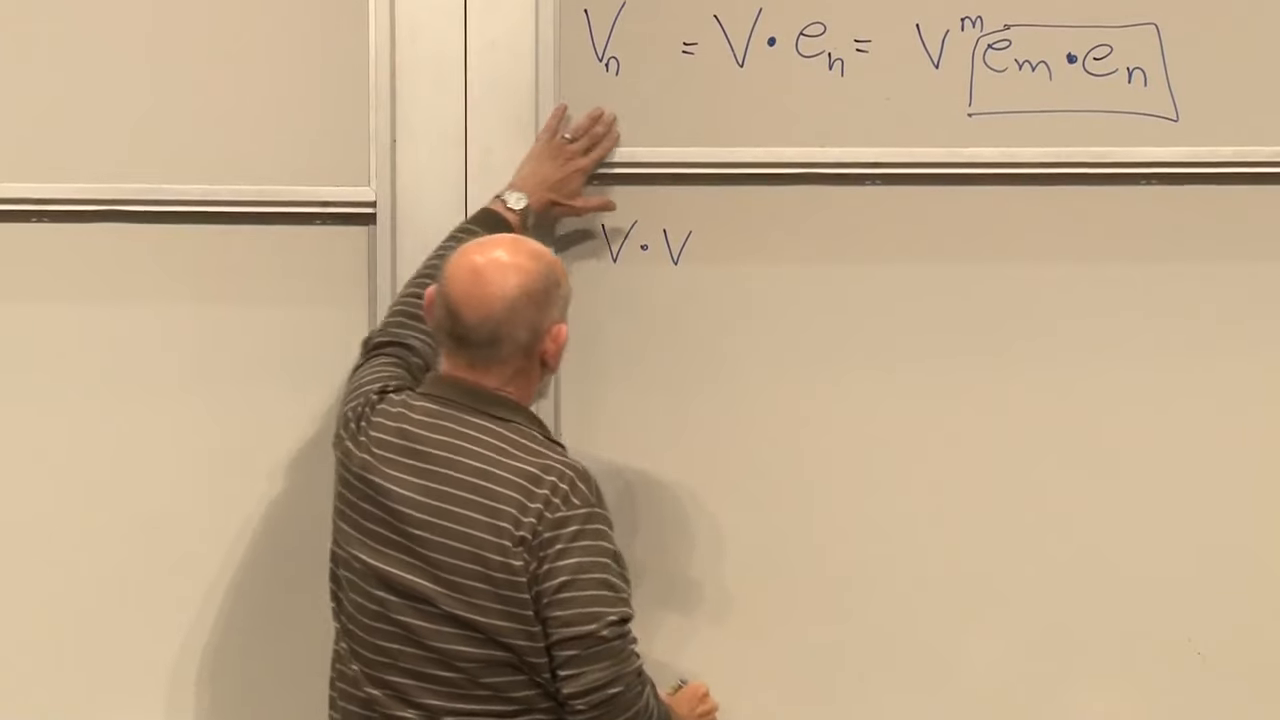
\includegraphics[width=\linewidth]{lecture_02_figure_07.png}
\caption{基底ベクトルのグラム行列としての計量。}
\lectureframe{00:23:40}
\end{figure}

同じ行列が長さを計算する：
\begin{align}
 \mathbf V\mathbin{\boldsymbol{\cdot}}\mathbf V
 &=(V^m\mathbf e_m)\mathbin{\boldsymbol{\cdot}}
   (V^n\mathbf e_n) \notag\\
 &=g_{mn}V^mV^n.
\label{eq:vector-length}
\end{align}

\begin{figure}[H]
\centering
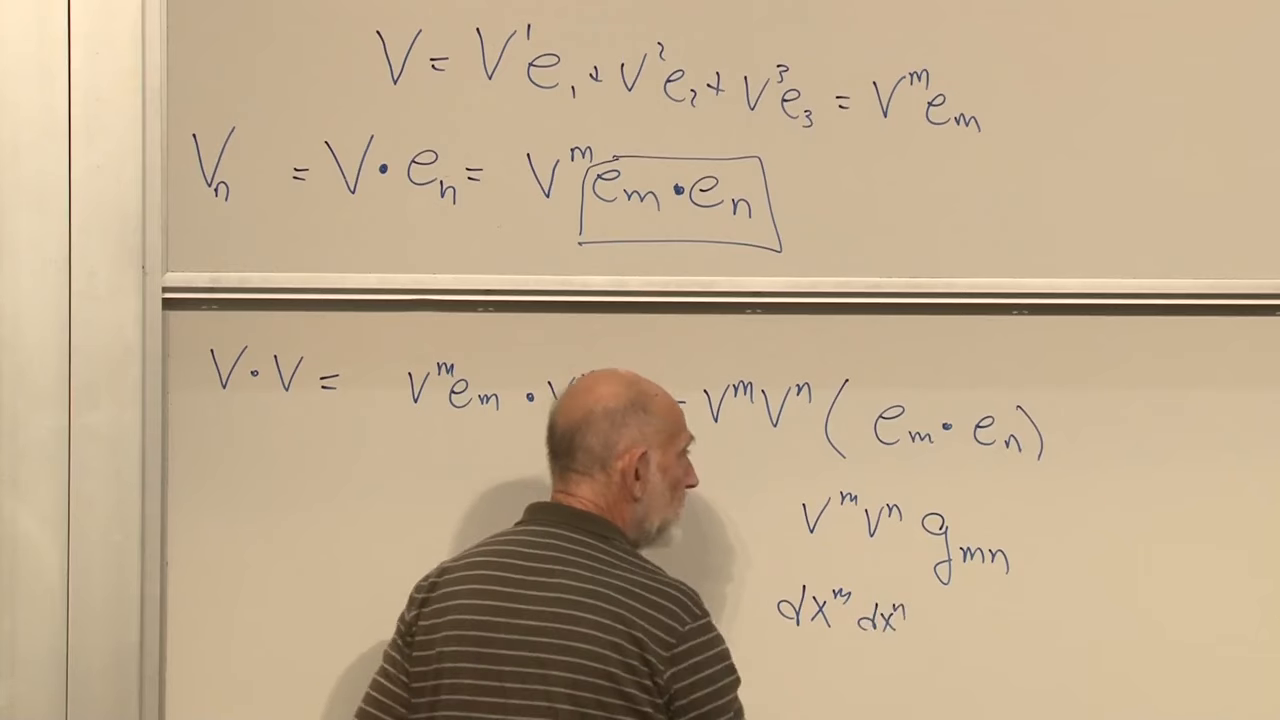
\includegraphics[width=\linewidth]{lecture_02_figure_08.png}
\caption{計量と反変成分を用いて表したベクトルのノルム。}
\lectureframe{00:25:00}
\end{figure}

\begin{classroomqa}
\audiencequestion{なぜ形式的な変換則の前にこの幾何学的構成を導入するのか。}
\lecturerresponse{それは添字に具体的な意味を与える。上付き成分は展開係数であり、下付き成分はベクトルの線形測定であり、計量が両者を結びつける。形式的な定義は、これらの役割が任意の滑らかな座標変換の下でも保たれることを教えてくれるだろう。\lecturetimestamp{00:26:07}}
\end{classroomqa}

\begin{classroomqa}
\audiencequestion{共変成分と反変成分が同じ数値をもつのはいつか。}
\lecturerresponse{正規直交ユークリッド基底では、
\(g_{mn}=\delta_{mn}\) であるから、\(V_m=V^m\) が成分ごとに成り立つ。単に直交しているだけでは十分ではない。基底ベクトルが単位長でなければ、対角計量は依然としてスケール因子を与える。
\lecturetimestamp{00:26:19}}
\end{classroomqa}

極座標は明快な警告を与える。動径方向と角度方向の座標線は直交して交わるが、固定された変化 \(d\theta\) は物理的距離 \(r\,d\theta\) に対応する。平面では、
\begin{equation}
 ds^2=dr^2+r^2d\theta^2,
\label{eq:polar-metric}
\end{equation}
したがって基底は直交しているがデカルトではない。

\begin{figure}[H]
\centering
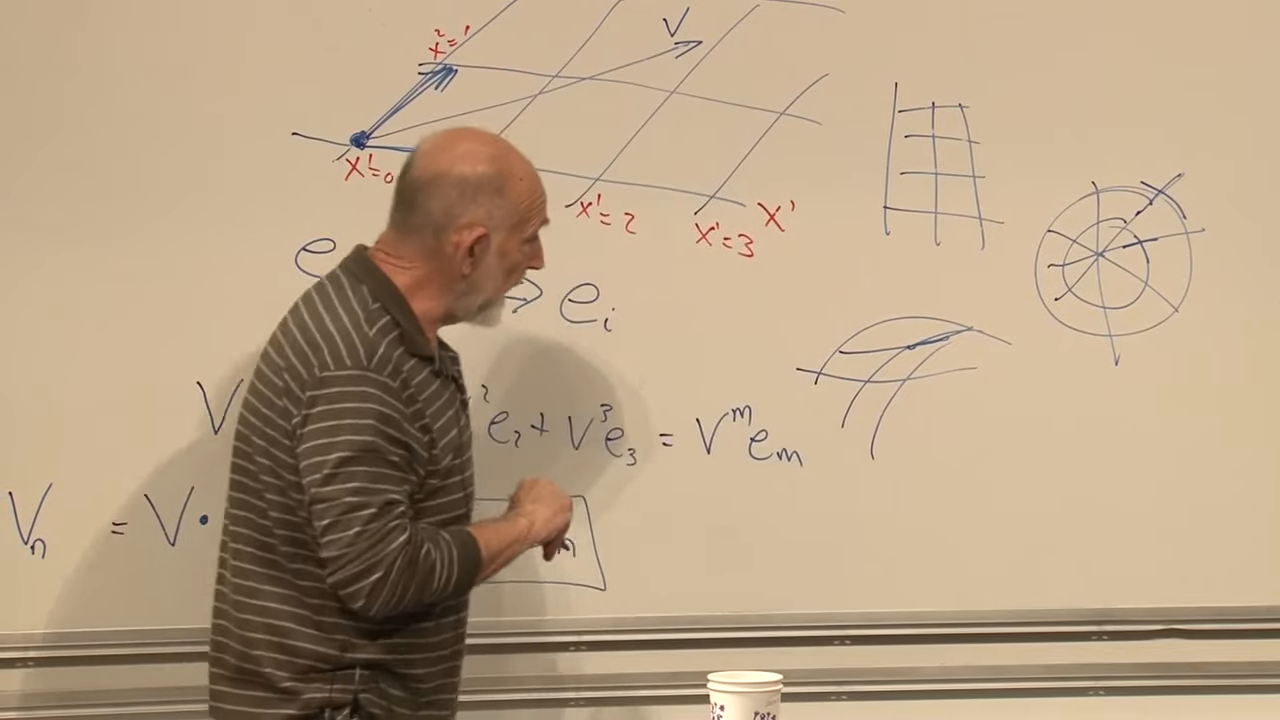
\includegraphics[width=\linewidth]{lecture_02_figure_09.png}
\caption{極座標：動径とともに増大する角度スケール因子をもつ直交座標方向。}
\lectureframe{00:28:10}
\end{figure}

\begin{classroomqa}
\audiencequestion{共変ベクトルは本当に異なるベクトルなのか、それとも同じベクトルを列挙する第二の方法にすぎないのか。}
\lecturerresponse{計量が与えられる前は、ベクトルと余ベクトルは異なる種類の線形対象である。ベクトルは接空間に属し、余ベクトルはその空間上の線形汎関数である。非退化計量は両者の間に一対一対応を与え、それは \(V_m=g_{mn}V^n\) で表されるが、その対応を同一視と取り違えてはならない。\lecturetimestamp{00:29:10}}
\end{classroomqa}

\section{変換則がテンソルを定義する}

最も安全な形式的定義は操作的である。配列がテンソルであるとは、その成分が適切なヤコビ因子によって変換することである。\eqref{eq:coordinate-maps} を微分すると
\begin{equation}
 dy^m=\frac{\partial y^m}{\partial x^n}\,dx^n.
\label{eq:differential-law}
\end{equation}
任意の反変ベクトルは同じ規則に従う：
\begin{equation}
 V'^m(y)
 =\frac{\partial y^m}{\partial x^n}V^n(x).
\label{eq:contravariant-law}
\end{equation}

\begin{figure}[H]
\centering
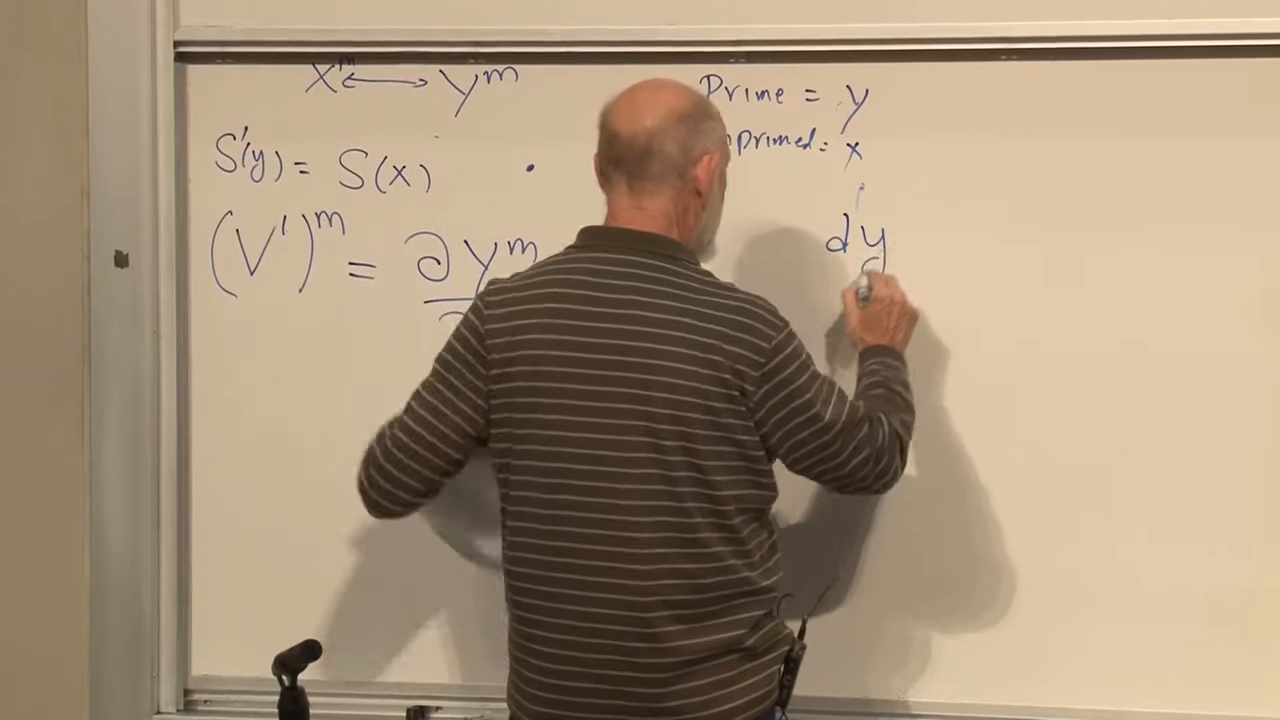
\includegraphics[width=\linewidth]{lecture_02_figure_10.png}
\caption{座標微分の変換をモデルとした反変変換則。}
\lectureframe{00:32:50}
\end{figure}

余ベクトルは逆ヤコビ行列で変換する：
\begin{equation}
 W'_m(y)
 =\frac{\partial x^n}{\partial y^m}W_n(x).
\label{eq:covariant-law}
\end{equation}
スカラーの勾配が標準的な例である。連鎖律を \eqref{eq:scalar-law} に適用すると、
\begin{equation}
 \frac{\partial S}{\partial y^m}
 =\frac{\partial x^n}{\partial y^m}
  \frac{\partial S}{\partial x^n}.
\label{eq:gradient-law}
\end{equation}

\begin{figure}[H]
\centering
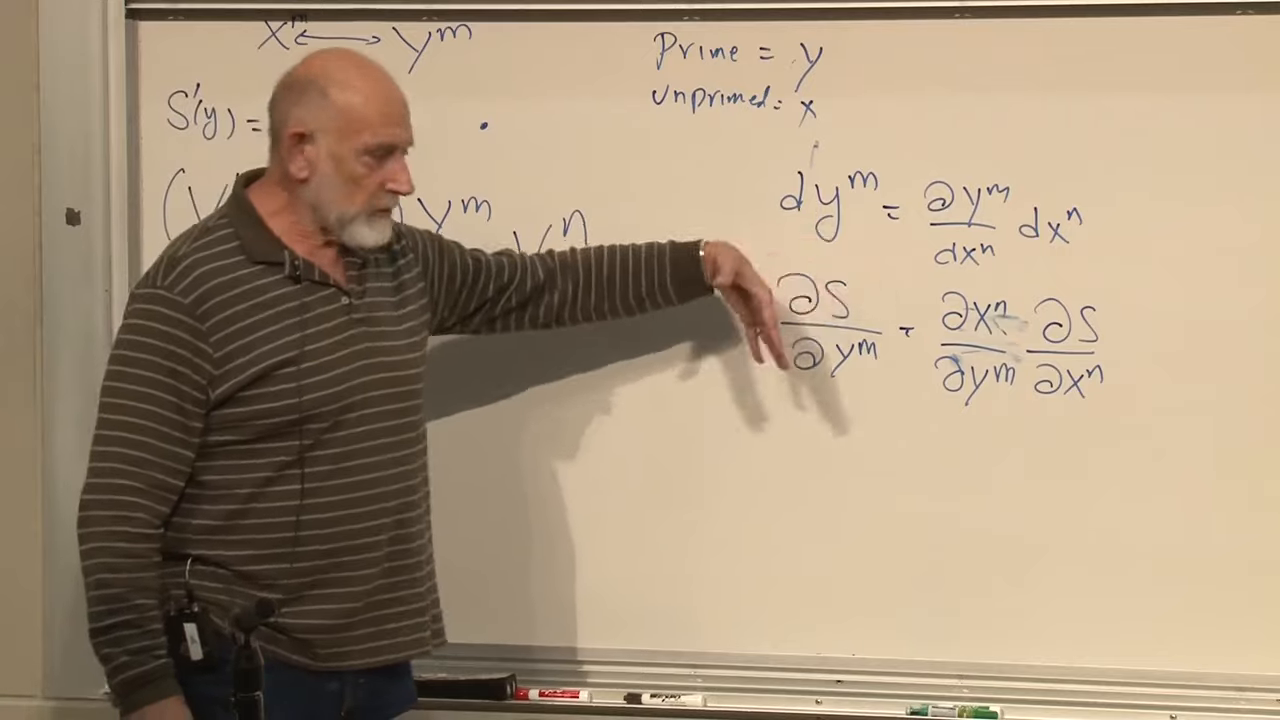
\includegraphics[width=\linewidth]{lecture_02_figure_11.png}
\caption{連鎖律によって余ベクトルとして変換するスカラー勾配。}
\lectureframe{00:34:20}
\end{figure}

\begin{classroomqa}
\audiencequestion{上付き成分と下付き成分は必ず同じ物理的単位をもつのか。}
\lecturerresponse{いいえ。座標成分は座標とその基底ベクトルの単位およびスケールの規約を受け継ぐ。一方の座標が長さで他方が角度であれば、それらの成分は次元すら共有する必要はない。物理的次元が座標に依存しない対象は、完全な縮約である。
\lecturetimestamp{00:35:41}}
\end{classroomqa}

\begin{classroomqa}
\audiencequestion{なぜ導関数は常微分ではなく偏微分なのか。}
\lecturerresponse{場は複数の座標に依存する。ヤコビ行列は、一つの引数が変化し他の引数が固定されているときに一つの座標関数がどのように変化するかを問うものである。したがってその成分は偏微分である。
\lecturetimestamp{00:36:45}}
\end{classroomqa}

このパターンは今や機械的に拡張される。上付きのプライム付き添字はそれぞれ\(\partial y/\partial x\)の因子を一つもたらし、下付きのプライム付き添字はそれぞれ\(\partial x/\partial y\)の因子を一つもたらす。混合テンソルは
\begin{equation}
 T'^m{}_n
 =
 \frac{\partial y^m}{\partial x^p}
 \frac{\partial x^q}{\partial y^n}
 T^p{}_q,
\label{eq:mixed-law}
\end{equation}
と変換し、二階の共変テンソルは
\begin{equation}
 W'_{mn}
 =
 \frac{\partial x^p}{\partial y^m}
 \frac{\partial x^q}{\partial y^n}
 W_{pq}.
\label{eq:rank-two-covariant-law}
\end{equation}
と変換する。

\begin{figure}[H]
\centering
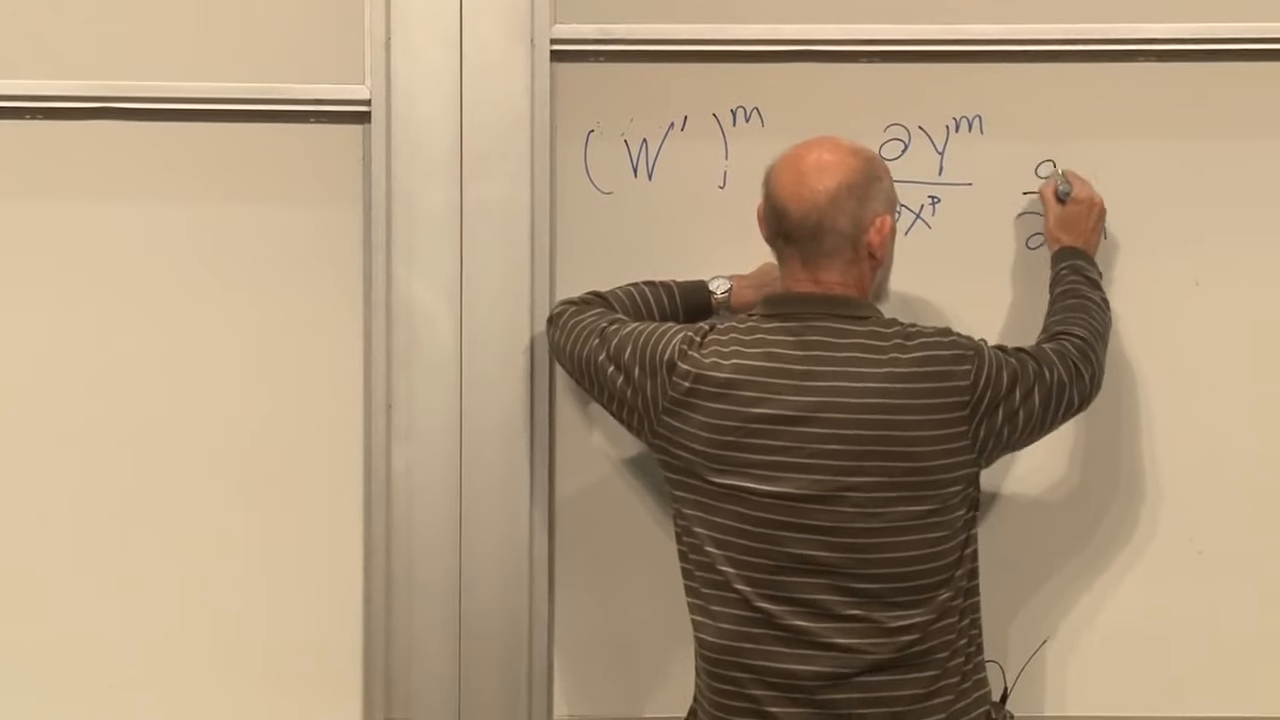
\includegraphics[width=\linewidth]{lecture_02_figure_12.png}
\caption{上付き添字を一つと下付き添字を一つもつテンソルの変換則。}
\lectureframe{00:40:45}
\end{figure}

\begin{figure}[H]
\centering
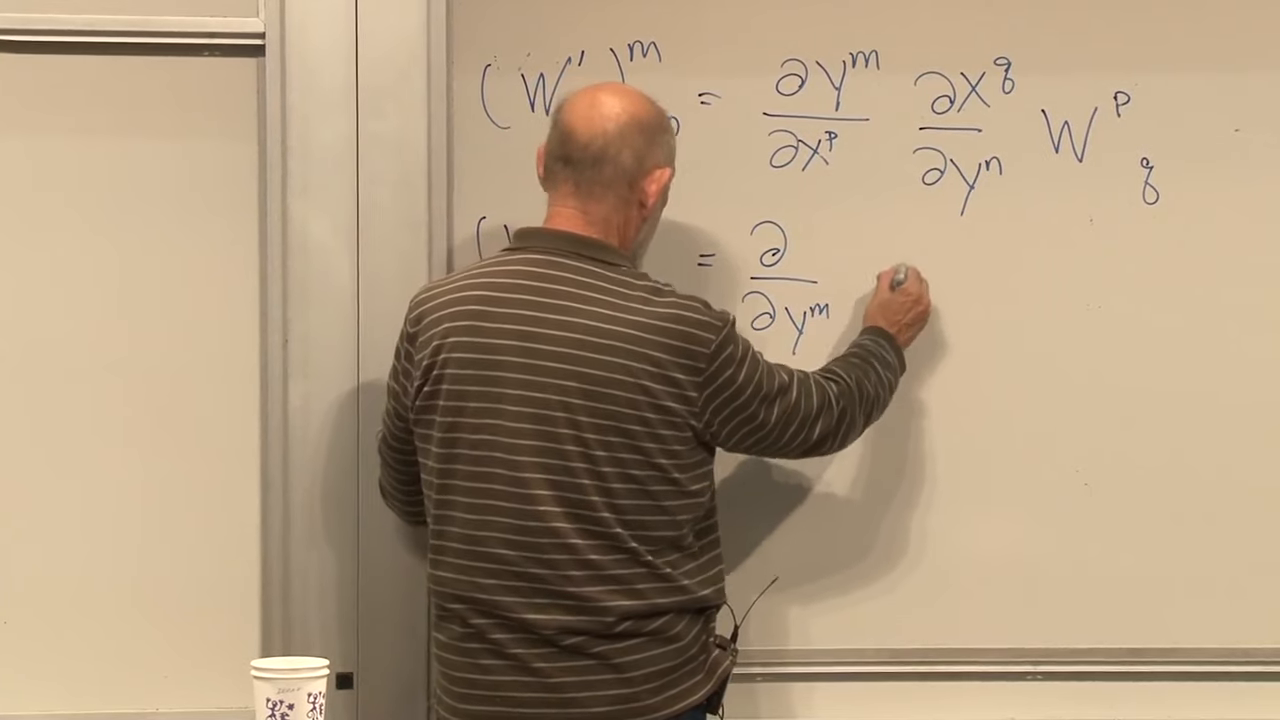
\includegraphics[width=\linewidth]{lecture_02_figure_13.png}
\caption{二階の共変変換則であり、各下付き添字に対してヤコビ行列の逆行列が一つずつ対応する。}
\lectureframe{00:42:15}
\end{figure}

特に断らない限り、繰り返された添字は和をとる。この規約は和の記号を除去しつつ、それを復元するのに必要なすべての情報を保持する。繰り返されるダミー添字は一つの項にちょうど二回、一度は上付き、一度は下付きで現れなければならない。自由添字は方程式の各項に一度ずつ現れる。

\begin{classroomqa}
\audiencequestion{この和の記法を導入したのは誰か。}
\lecturerresponse{慣例的にアインシュタインの功績とされ、それゆえアインシュタインの和の規約と呼ばれる。その価値は歴史的な装飾ではない。添字のパターンによって、許されるテンソル演算が一目で見えるようになる。\lecturetimestamp{00:43:21}}
\end{classroomqa}

\section{テンソル方程式と座標に依存しない真理}

成分は座標とともに変化するが、テンソル方程式はどの座標系でも成り立つ。同じ型の二つのテンソルが\(W=T\)を満たすならば、それらの差はゼロテンソルである。
\begin{equation}
 W^{m\cdots}{}_{\cdots n}
 -T^{m\cdots}{}_{\cdots n}=0.
\label{eq:tensor-equality}
\end{equation}
変換則は線形であるから、一つの系でゼロの成分はどの系でもゼロの成分を与える。両辺の自由添字が一致していることは不可欠である。異なるテンソル型の対象の間の方程式には座標に依存しない意味はない。

\begin{figure}[H]
\centering
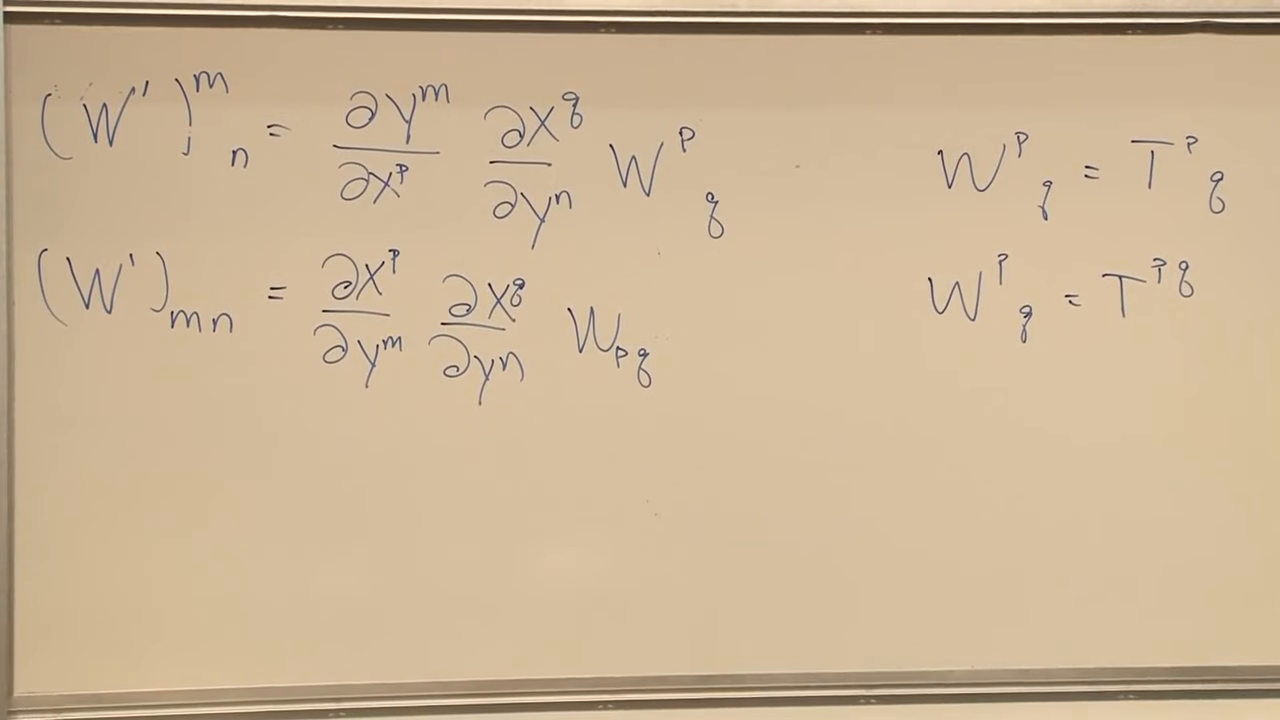
\includegraphics[width=\linewidth]{lecture_02_figure_14.png}
\caption{添字構造の一致が、成分の等しさをどの座標系でも成り立つテンソル方程式に変える。}
\lectureframe{00:46:35}
\end{figure}

\begin{classroomqa}
\audiencequestion{ベクトルの成分が変化しているなら、正確には何が不変なのか。}
\lecturerresponse{幾何学的テンソルとテンソル方程式の真理が不変であり、座標のリストは不変ではない。スカラーは添字をもたない特別な場合であり、したがってある点におけるその数値はどの座標系でも同じである。\lecturetimestamp{00:47:19}}
\end{classroomqa}

\begin{classroomqa}
\audiencequestion{ベクトルの大きさが不変な対応物であり、大きさがゼロならベクトルはゼロであるのか。}
\lecturerresponse{計量が与えられれば、縮約\(g_{mn}V^mV^n\)はスカラーであり、したがって不変なノルムの二乗である。正定値幾何学ではそれはゼロベクトルに対してのみ消える。ローレンツ時空では非零のヌルベクトルがゼロのノルムをもちうるので、この二つの主張は区別して保たなければならない。\lecturetimestamp{00:48:04}}
\end{classroomqa}

\section{テンソルに許される代数}

黒板には、必要となる主要な演算がまとめられている。スカラーによる乗法、同じ型のテンソルの加減、テンソル積の形成、上付き添字と下付き添字の縮約、そして最終的には共変微分である。

\begin{figure}[H]
\centering
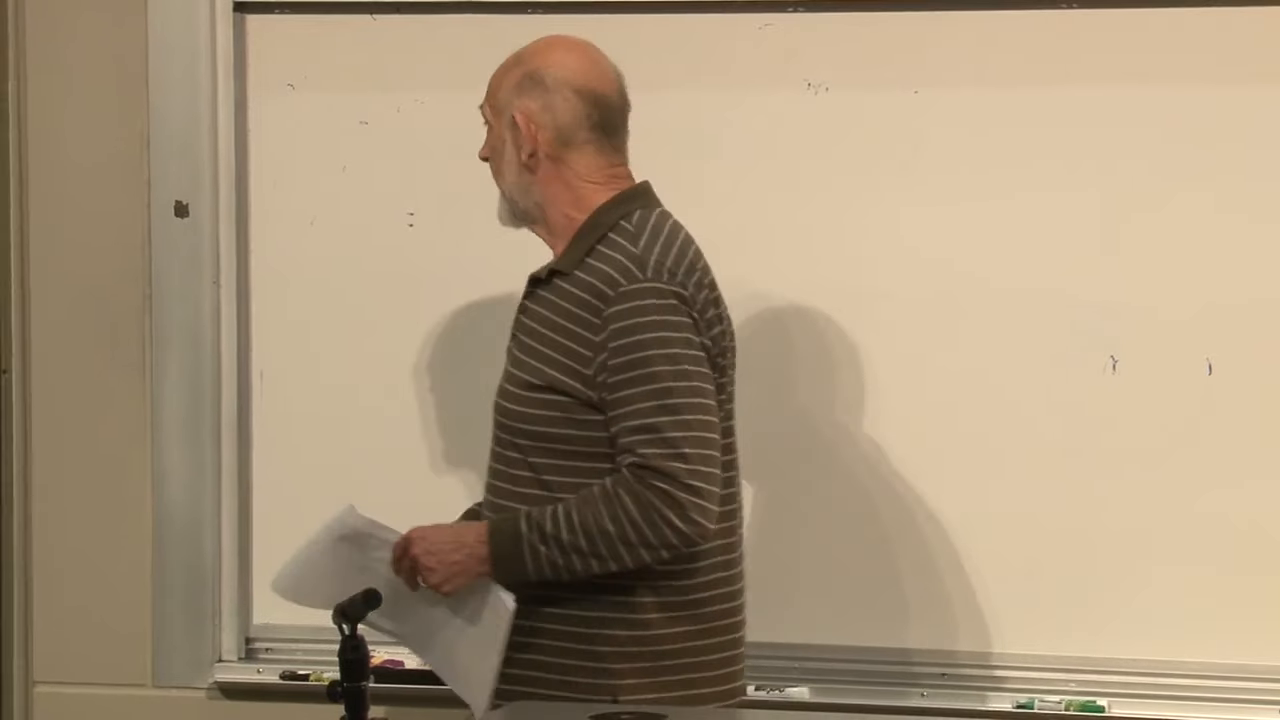
\includegraphics[width=\linewidth]{lecture_02_figure_15.png}
\caption{テンソル演算の黒板一覧：加法、乗法、縮約、微分。}
\lectureframe{00:50:40}
\end{figure}

\begin{classroomqa}
\audiencequestion{何に関する微分か。}
\lecturerresponse{位置に関して、したがって座標に関してである。通常の成分の微分は、ヤコビ行列自体が変化するため、一般にはテンソルとして変換しない。共変微分はこれを修復するが、その構成は幾何学の準備が整うまで延期される。\lecturetimestamp{00:51:49}}
\end{classroomqa}

スカラー倍は直ちにできる。加法と減法はテンソル型の一致を必要とする。
\begin{equation}
 C^m{}_n=A^m{}_n+B^m{}_n,
\qquad
 D^m{}_n=A^m{}_n-B^m{}_n.
\label{eq:tensor-addition}
\end{equation}
ベクトルを余ベクトルに加えたり、二階のテンソルをスカラーに加えたりすることはできない。ちょうど、速度を面積に加えることができないのと同じである。

\begin{figure}[H]
\centering
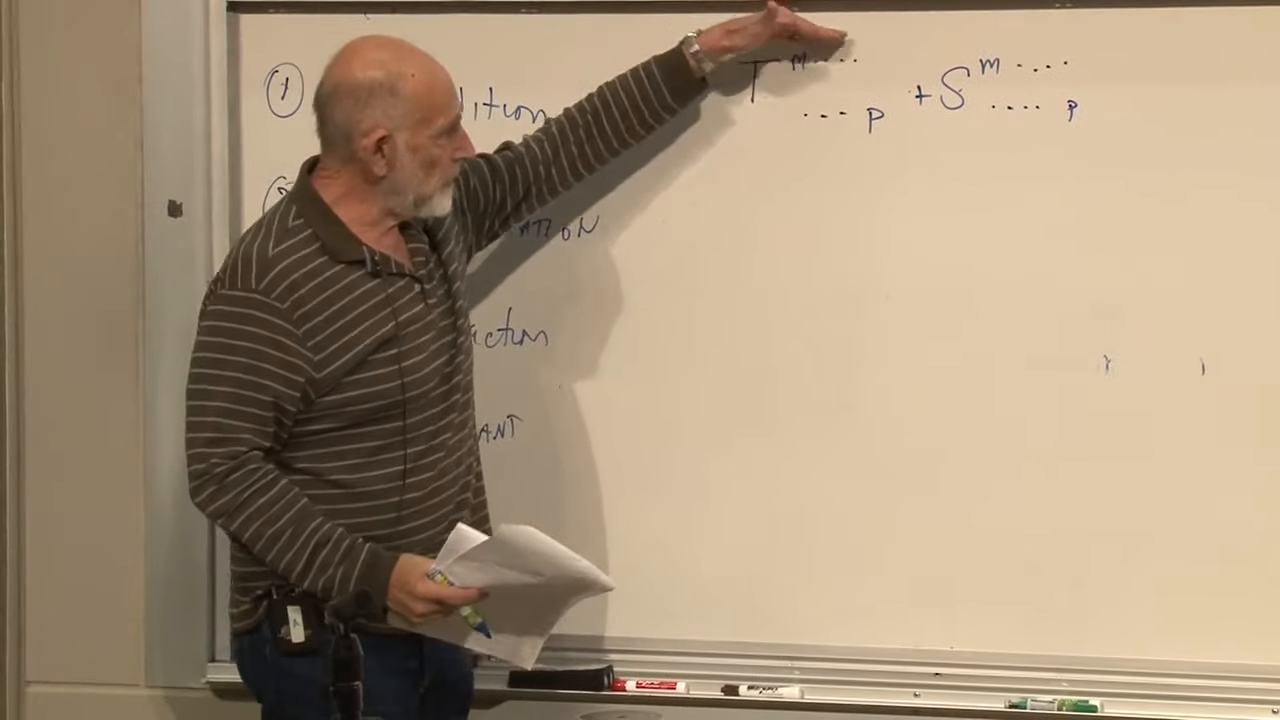
\includegraphics[width=\linewidth]{lecture_02_figure_16.png}
\caption{加法は、同じ自由添字パターンをもつテンソルに対してのみ成分ごとに定義される。}
\lectureframe{00:53:00}
\end{figure}

テンソル積はその因子のすべての添字を結合する。例えば、
\begin{equation}
 T^{mn}=V^mW^n,
\qquad
 S^m{}_n=V^mU_n.
\label{eq:tensor-products}
\end{equation}
四次元では\(T^{mn}\)は十六個の成分をもつ。どの添字も和をとられていないので、これは内積ではなく外積である。

\begin{figure}[H]
\centering
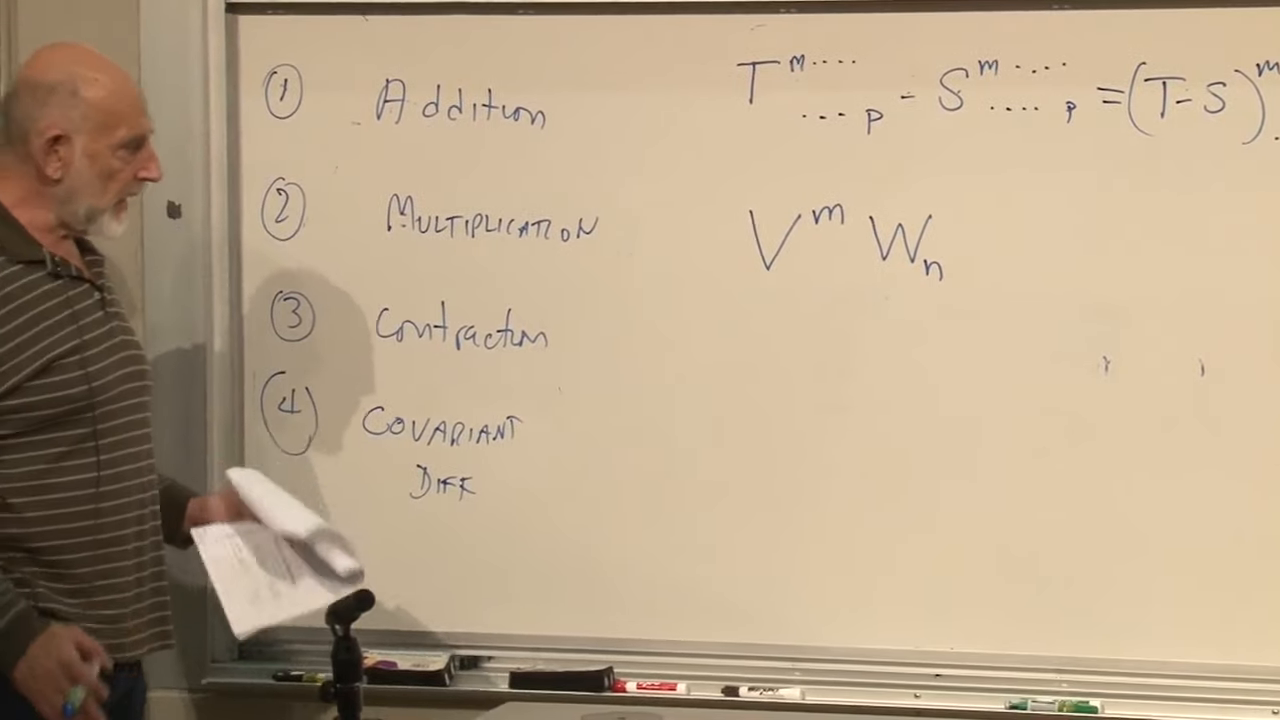
\includegraphics[width=\linewidth]{lecture_02_figure_17.png}
\caption{各ベクトル因子から一つの自由添字を保持するテンソル積。}
\lectureframe{00:55:15}
\end{figure}

\begin{classroomqa}
\audiencequestion{ここで二つのベクトルの積とは内積のことか。}
\lecturerresponse{いいえ。内積は一つの添字を縮約してスカラーを生じる。テンソル積は両方の添字を自由のまま残すので、階数2のテンソルを生じる。四次元ではそれは一成分ではなく十六成分である。\lecturetimestamp{00:56:36}}
\end{classroomqa}

\begin{classroomqa}
\audiencequestion{成分の数は可換だから、二つのベクトル因子を入れ替えても違いは生じないのか。}
\lecturerresponse{通常のスカラー成分については、
\(V^mW^n=W^nV^m\)。しかしテンソルの枠は順序づけられている。因子を入れ替えたうえで第一の枠を\(m\)、第二の枠を\(n\)と名付けると、転置された配列が得られる。\(T^{mn}\)は\(T^{nm}\)に等しいとは限らない。
\lecturetimestamp{00:58:52}}
\end{classroomqa}

\section{縮約と逆ヤコビアンの補題}

縮約の鍵は連鎖律である。座標写像が互いに逆であることから、
\begin{equation}
 \frac{\partial x^b}{\partial y^m}
 \frac{\partial y^m}{\partial x^a}
 =
 \frac{\partial x^b}{\partial x^a}
 =\delta^b{}_a.
\label{eq:inverse-jacobian}
\end{equation}
二つのヤコビ行列は互いに逆であり、その積はクロネッカーのデルタである。

\begin{figure}[H]
\centering
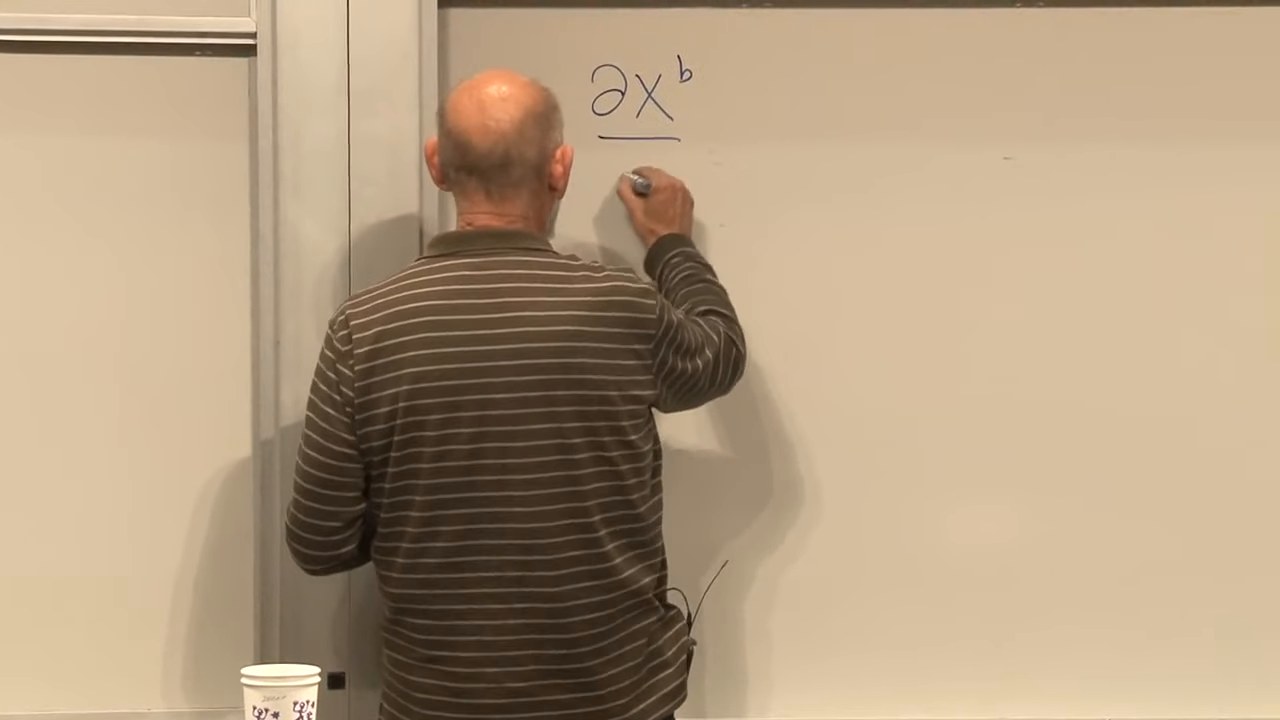
\includegraphics[width=\linewidth]{lecture_02_figure_18.png}
\caption{テンソルの縮約の背後にある補題として準備された逆ヤコビアンの恒等式。}
\lectureframe{01:02:15}
\end{figure}

\begin{classroomqa}
\audiencequestion{逆ヤコビアンとはどのような対象か。}
\lecturerresponse{それは逆座標写像の導関数行列である。その成分は\(\partial x^b/\partial y^m\)であり、\(\partial y^m/\partial x^a\)との行列積は多変数の連鎖律により単位行列を与える。\lecturetimestamp{01:02:37}}
\end{classroomqa}

簡単な証明が記法を明快にする。任意のスカラー関数\(f\)について、
\begin{equation}
 \frac{\partial f}{\partial y^m}
 \frac{\partial y^m}{\partial x^a}
 =\frac{\partial f}{\partial x^a}.
\end{equation}
\(f=x^b\)と選ぶと、
\begin{equation}
 \frac{\partial x^b}{\partial y^m}
 \frac{\partial y^m}{\partial x^a}
 =\frac{\partial x^b}{\partial x^a}
 =\delta^b{}_a.
\end{equation}

\begin{figure}[H]
\centering
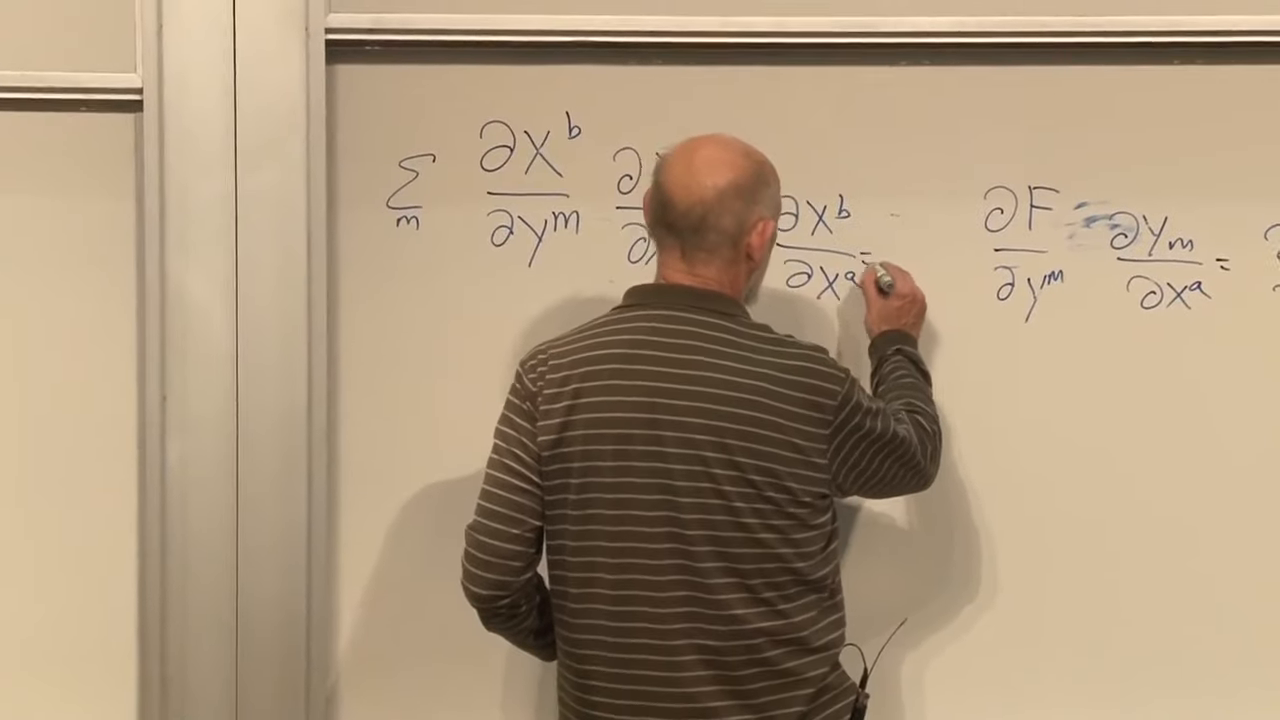
\includegraphics[width=\linewidth]{lecture_02_figure_19.png}
\caption{連鎖律により逆ヤコビアンがクロネッカーのデルタに縮まる。}
\lectureframe{01:04:55}
\end{figure}

\begin{classroomqa}
\audiencequestion{\(\delta^b{}_a\)が単位行列となるのはデカルト座標においてのみか。}
\lecturerresponse{いいえ。混合テンソル\(\delta^b{}_a\)はあらゆる座標系において単位写像を表す。\(\delta_{ab}\)と書かれるユークリッド計量は正規直交デカルト座標に特有であるが、混合添字の単位行列をその計量と混同してはならない。
\lecturetimestamp{01:04:58}}
\end{classroomqa}

次に混合テンソル\(T^m{}_n\)を取る。その変換されたトレースは
\begin{align}
 T'^m{}_m
 &=
 \frac{\partial y^m}{\partial x^a}
 \frac{\partial x^b}{\partial y^m}
 T^a{}_b \notag\\
 &=\delta^b{}_aT^a{}_b
 =T^a{}_a.
\label{eq:trace-invariant}
\end{align}
縮約された量は自由添字を持たないので、スカラーである。

\begin{figure}[H]
\centering
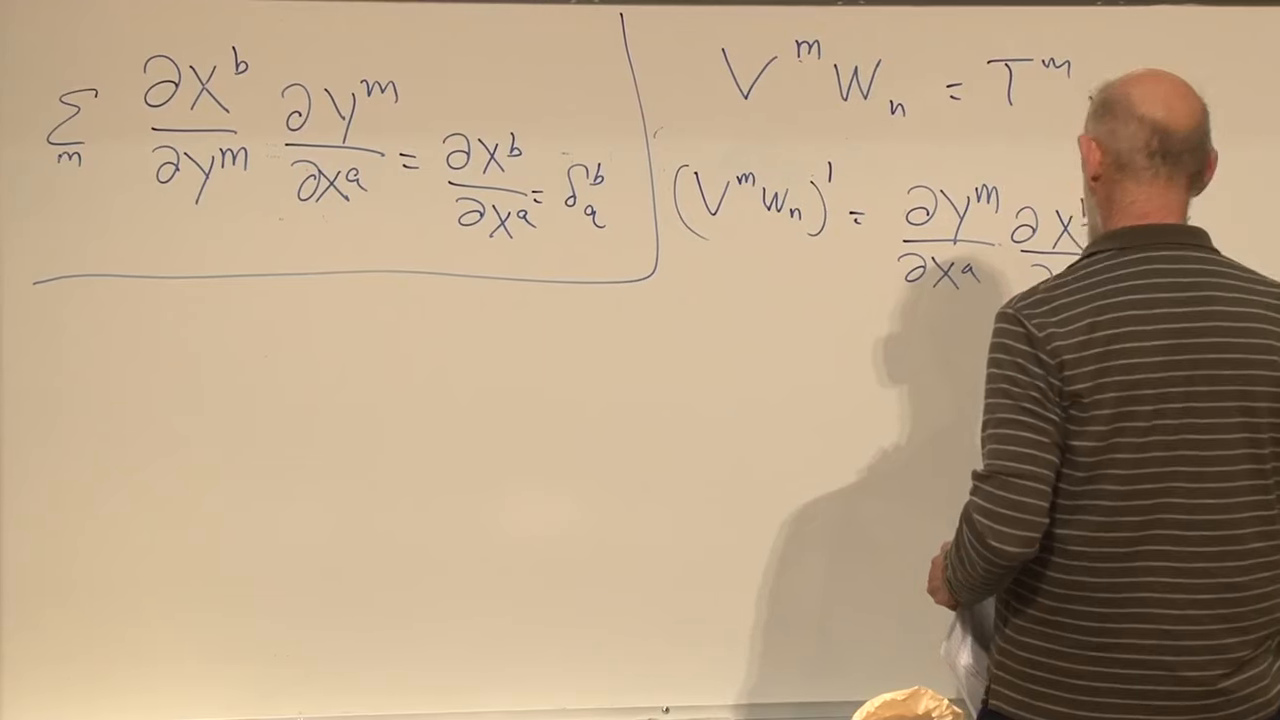
\includegraphics[width=\linewidth]{lecture_02_figure_20.png}
\caption{上添字と下添字を縮約する前の混合テンソルの変換。}
\lectureframe{01:07:45}
\end{figure}

\begin{figure}[H]
\centering
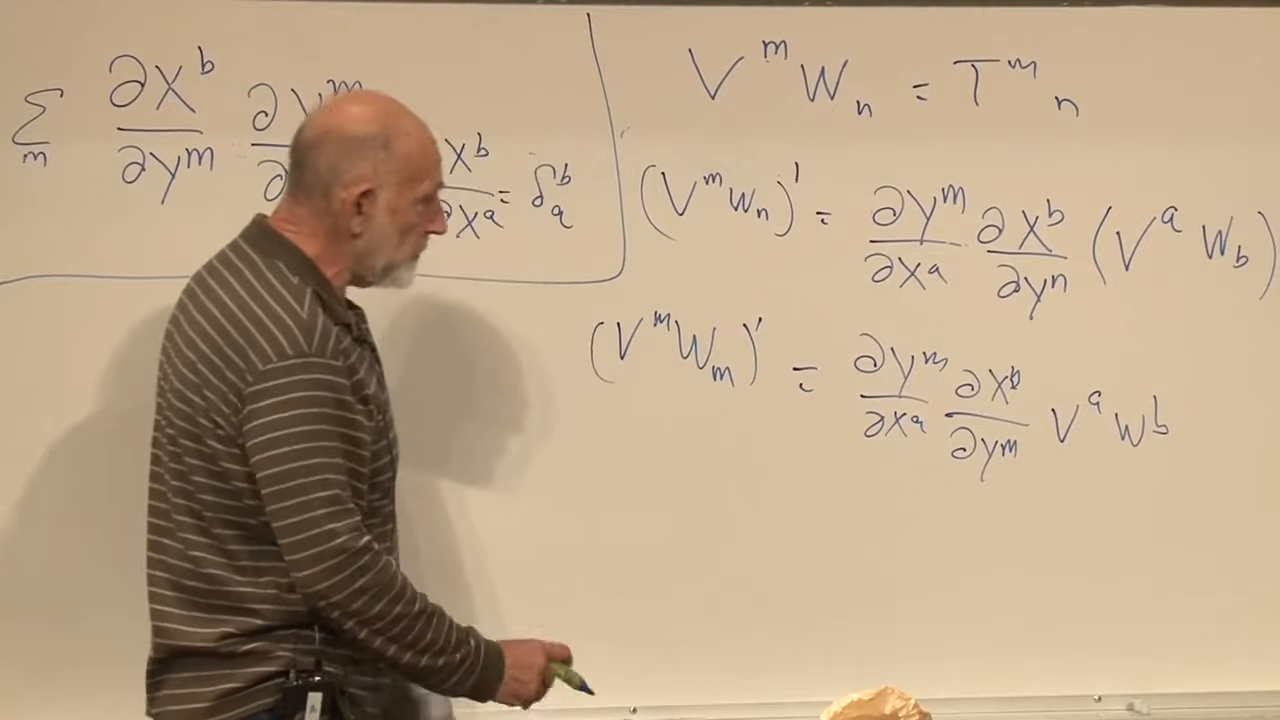
\includegraphics[width=\linewidth]{lecture_02_figure_21.png}
\caption{縮約の下でヤコビアンが相殺し、どちらの座標系でも同じスカラーのトレースが残る。}
\lectureframe{01:10:30}
\end{figure}

\begin{classroomqa}
\audiencequestion{縮約の後、結果は依然として添字を持つのか。}
\lecturerresponse{縮約された対だけが消える。\(T^m{}_n\)の唯一の上添字と下添字を縮約するとスカラーが残る。より高階のテンソルでは、縮約されていないすべての添字が自由のまま残る。
\lecturetimestamp{01:09:00}}
\end{classroomqa}

例えば、
\begin{equation}
 A^{mn}{}_{pq}
 \longmapsto
 A^{mn}{}_{pn}
 =B^m{}_p
\label{eq:higher-rank-contraction}
\end{equation}
は\(n\)を縮約し、階数を二だけ下げる。具体的な文字はダミーラベルであり、構造上の規則は一つの上添字の枠と一つの下添字の枠が和を取られることである。

\begin{figure}[H]
\centering
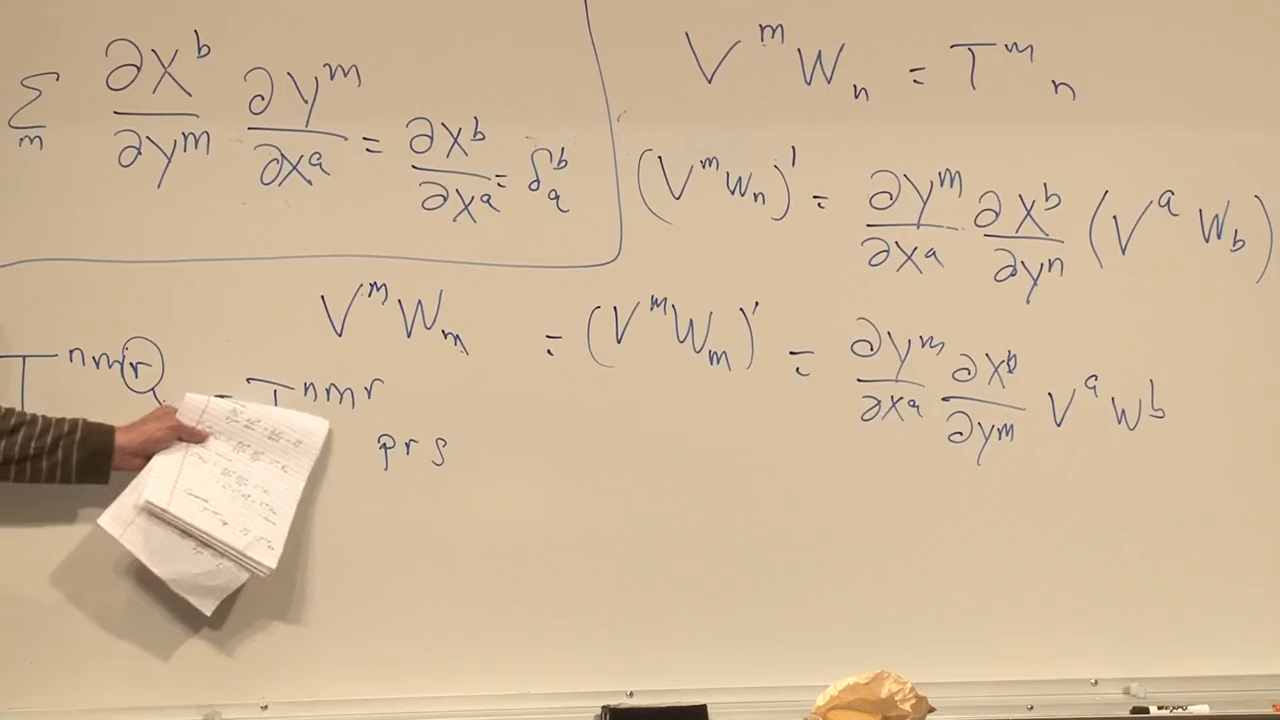
\includegraphics[width=\linewidth]{lecture_02_figure_22.png}
\caption{より高階の縮約は一つの上添字と一つの下添字を取り除き、残りの自由添字を保つ。}
\lectureframe{01:12:35}
\end{figure}

\begin{classroomqa}
\audiencequestion{なぜ二つの上添字、あるいは二つの下添字を同じように縮約してはならないのか。}
\lecturerresponse{二つの上添字は同じ向きの二つのヤコビアン、
\(\partial y^m/\partial x^a\)と
\(\partial y^m/\partial x^b\)を与える。それらは掛け合わさって単位行列にはならないので、提案された和はテンソルの変換則を持たない。計量によってまず一方の添字を下げることができ、その後なら上--下の縮約は合法である。その追加のテンソルがなければ、この操作は座標不変ではない。\lecturetimestamp{01:13:03}}
\end{classroomqa}

\begin{figure}[H]
\centering
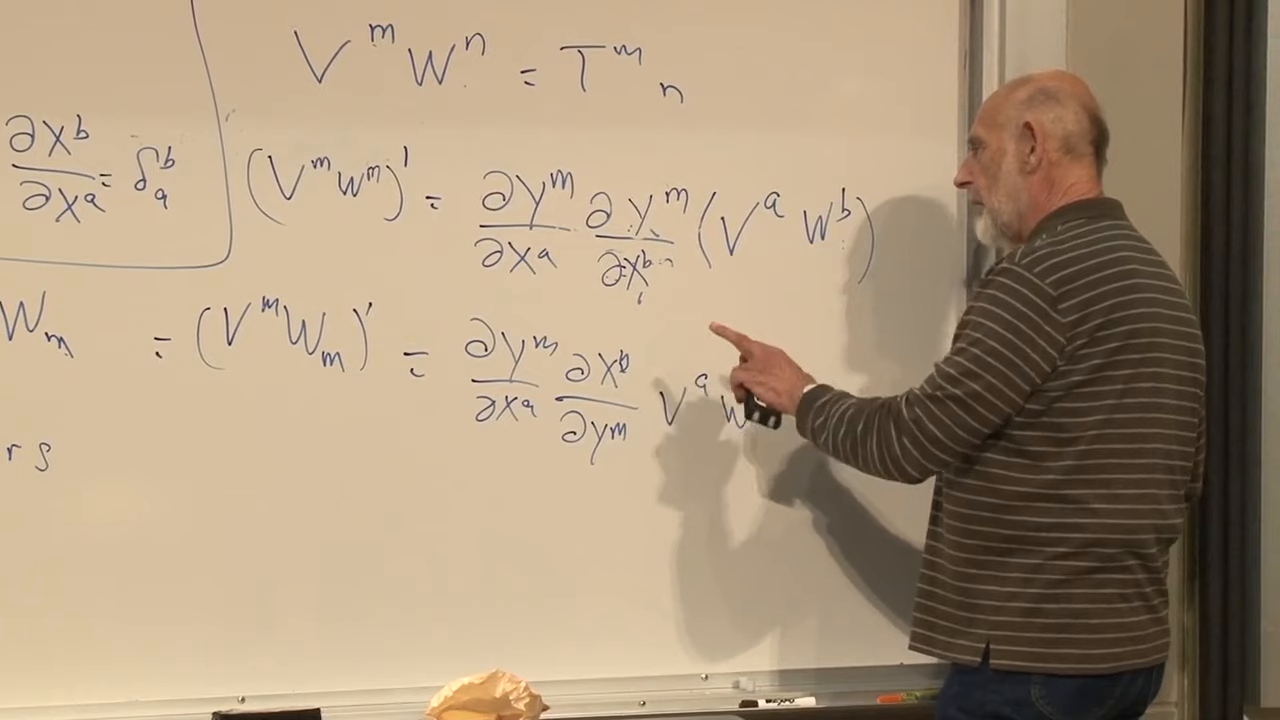
\includegraphics[width=\linewidth]{lecture_02_figure_23.png}
\caption{同じ反変性の縮約を試みると、同じ向きの二つのヤコビアンが残るため、単位行列に縮まらない。}
\lectureframe{01:14:30}
\end{figure}

\begin{classroomqa}
\audiencequestion{縮約は内積のテンソル版か。}
\lecturerresponse{縮約はベクトルの枠と余ベクトルの枠を対にし、基本的な不変の対を作る。計量があれば、二つのベクトルをそのような対に変えることができるので、よく知られた内積は計量に続く縮約である。\lecturetimestamp{01:14:43}}
\end{classroomqa}

\begin{classroomqa}
\audiencequestion{縮約される二つの添字は同じ範囲を走らなければならないのか。}
\lecturerresponse{はい。それらは同じ\(d\)次元の接空間と余接空間の双対基底を指す。そうでなければ、和と逆ヤコビアンの恒等式は定義されないであろう。
\lecturetimestamp{01:15:13}}
\end{classroomqa}

\begin{classroomqa}
\audiencequestion{一つの座標系で消えるテンソルは、なぜどの座標系でも消えるのか。}
\lecturerresponse{変換された各成分は、もとの成分の線形結合である。すべての入力成分がゼロであれば、それらの結合はすべて消える。この単純な線形性が、テンソル方程式を座標に依存しないものにしている。\lecturetimestamp{01:15:31}}
\end{classroomqa}

\section{二乗距離から計量へ}

ここで幾何学に戻る。成分\(dx^m\)をもつ無限小変位に対し、その二乗長を次で定義する。
\begin{equation}
 ds^2=g_{mn}(x)\,dx^m dx^n.
\label{eq:line-element}
\end{equation}
これは一般化されたピタゴラスの定理である。計量は点ごとに変化してよく、非対角項は座標方向の非直交性を記録する。

\begin{figure}[H]
\centering
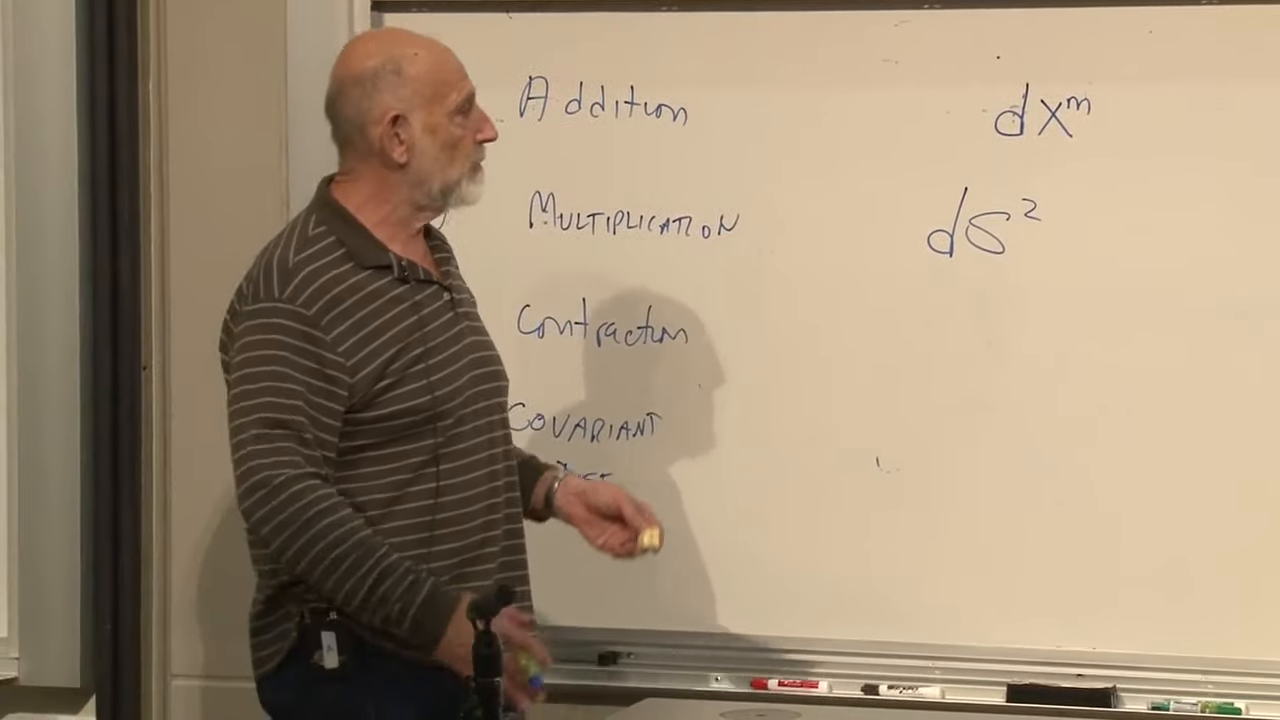
\includegraphics[width=\linewidth]{lecture_02_figure_24.png}
\caption{テンソル演算の一覧に代わって、無限小線素の二次定義が現れる。}
\lectureframe{01:18:45}
\end{figure}

\(dx^m dx^n=dx^n dx^m\)であるから、対称部分のみが寄与する。したがって次をとってよい。
\begin{equation}
 g_{mn}=g_{nm}.
\label{eq:metric-symmetry}
\end{equation}
\(d\)次元では、対称計量は
\begin{equation}
 \frac{d(d+1)}{2}
\label{eq:metric-component-count}
\end{equation}
個の独立成分をもつ。すなわち四次元では十個、三次元では六個、二次元では三個である。

\begin{figure}[H]
\centering
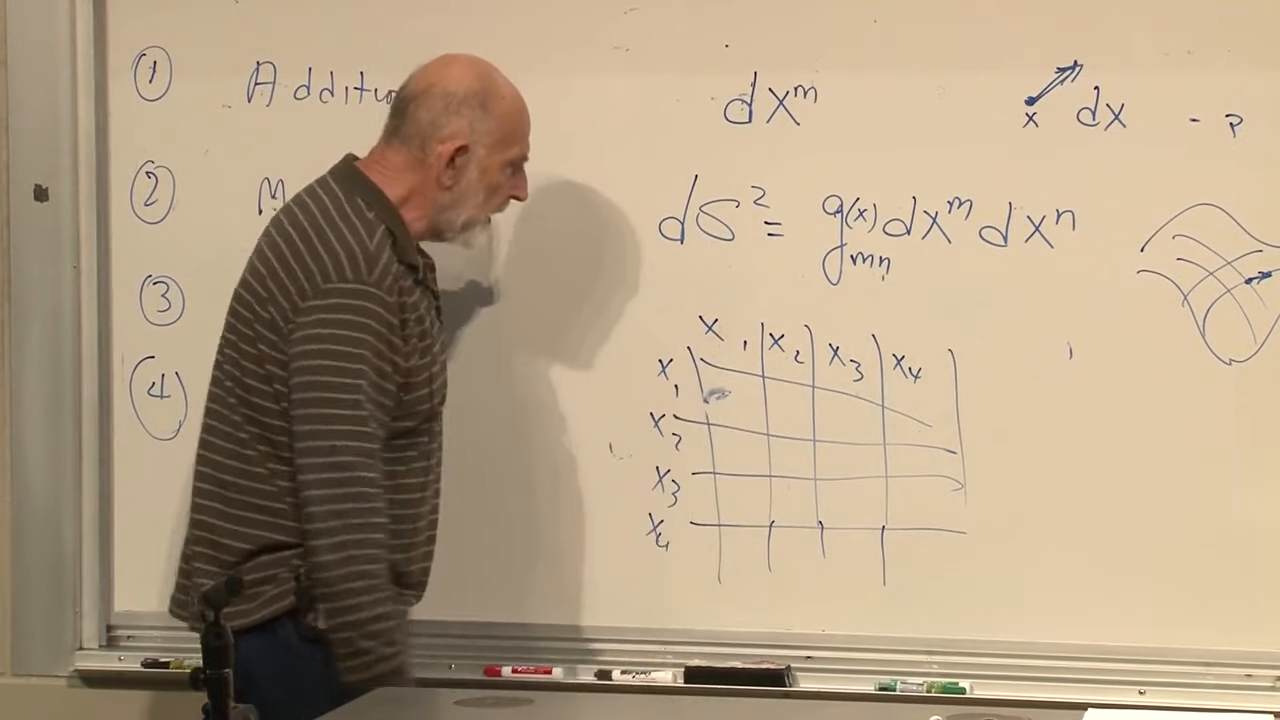
\includegraphics[width=\linewidth]{lecture_02_figure_25.png}
\caption{線素と、計量の独立な成分を数えるために用いられる対称成分の配列。}
\lectureframe{01:21:35}
\end{figure}

\begin{classroomqa}
\audiencequestion{四次元で独立な計量成分が十六個ではなく十個であるのはなぜか。}
\lecturerresponse{対角成分が四つあり、非対角の順序を問わない対が六つある。同値に、
\(4(4+1)/2=10\)である。反対称部分は対称積\(dx^m dx^n\)に掛かり、相殺される。\lecturetimestamp{01:19:50}}
\end{classroomqa}

\begin{classroomqa}
\audiencequestion{三次元では独立な成分はいくつあるか。}
\lecturerresponse{六個である。対角成分が三つ、非対角の対が三つ、すなわち\(3(3+1)/2\)である。\lecturetimestamp{01:20:47}}
\end{classroomqa}

\begin{classroomqa}
\audiencequestion{二次元ではどうか。}
\lecturerresponse{三つである。\(g_{11}\)、\(g_{22}\)、および唯一の対称な対\(g_{12}=g_{21}\)である。\lecturetimestamp{01:22:28}}
\end{classroomqa}

\subsection{計量がテンソルである理由}

二乗距離はスカラーである。したがって同じ変位を二つの座標系で書くと、
\begin{equation}
 g_{mn}(x)\,dx^m dx^n
 =
 g'_{pq}(y)\,dy^pdy^q.
\label{eq:length-invariance}
\end{equation}
となる。
\begin{equation}
 dx^m=\frac{\partial x^m}{\partial y^p}\,dy^p
\end{equation}
を二度用いると、
\begin{align}
 ds^2
 &=
 g_{mn}(x)
 \frac{\partial x^m}{\partial y^p}
 \frac{\partial x^n}{\partial y^q}
 dy^pdy^q.
\label{eq:metric-transform-derivation}
\end{align}
となる。プライム付きの表式と比較すると、
\begin{equation}
 g'_{pq}(y)
 =
 \frac{\partial x^m}{\partial y^p}
 \frac{\partial x^n}{\partial y^q}
 g_{mn}(x).
\label{eq:metric-transformation}
\end{equation}
が同定される。これはまさに共変二階テンソルの変換則である。

\begin{figure}[H]
\centering
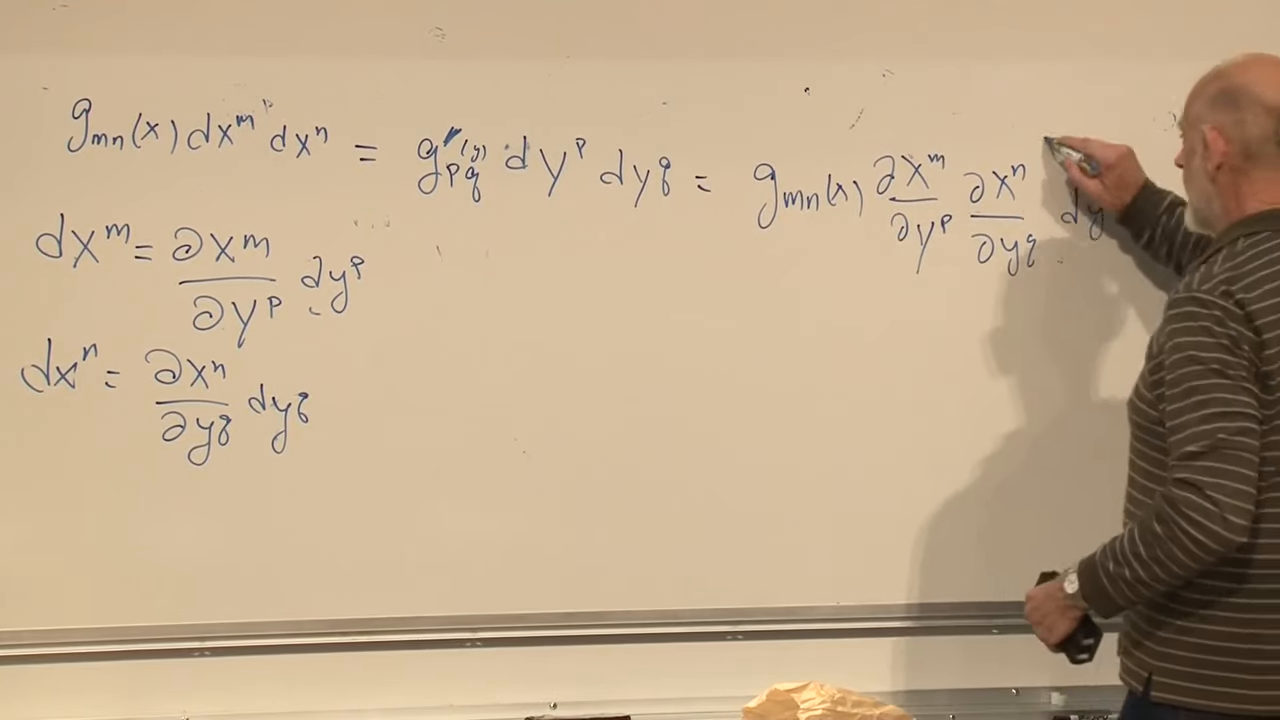
\includegraphics[width=\linewidth]{lecture_02_figure_26.png}
\caption{スカラー線素の不変性からの計量変換則の導出。}
\lectureframe{01:26:25}
\end{figure}

この結論は二つの下付き添字の理由も説明する。計量の各下付き添字は、変位成分が担う一つの上付き添字と対になる。座標変換の下で、\eqref{eq:metric-transformation}における二つの逆ヤコビアンが、微分の二つの順ヤコビアンを打ち消し、\(ds^2\)を不変に保つ。

\section{計量行列とその逆行列}

ある点において、\(g_{mn}\)は対称行列である。
\begin{equation}
 [g_{mn}]
 =
 \begin{pmatrix}
 g_{11} & g_{12} & \cdots \\
 g_{12} & g_{22} & \cdots \\
 \vdots & \vdots & \ddots
 \end{pmatrix}.
\label{eq:metric-matrix}
\end{equation}

\begin{figure}[H]
\centering
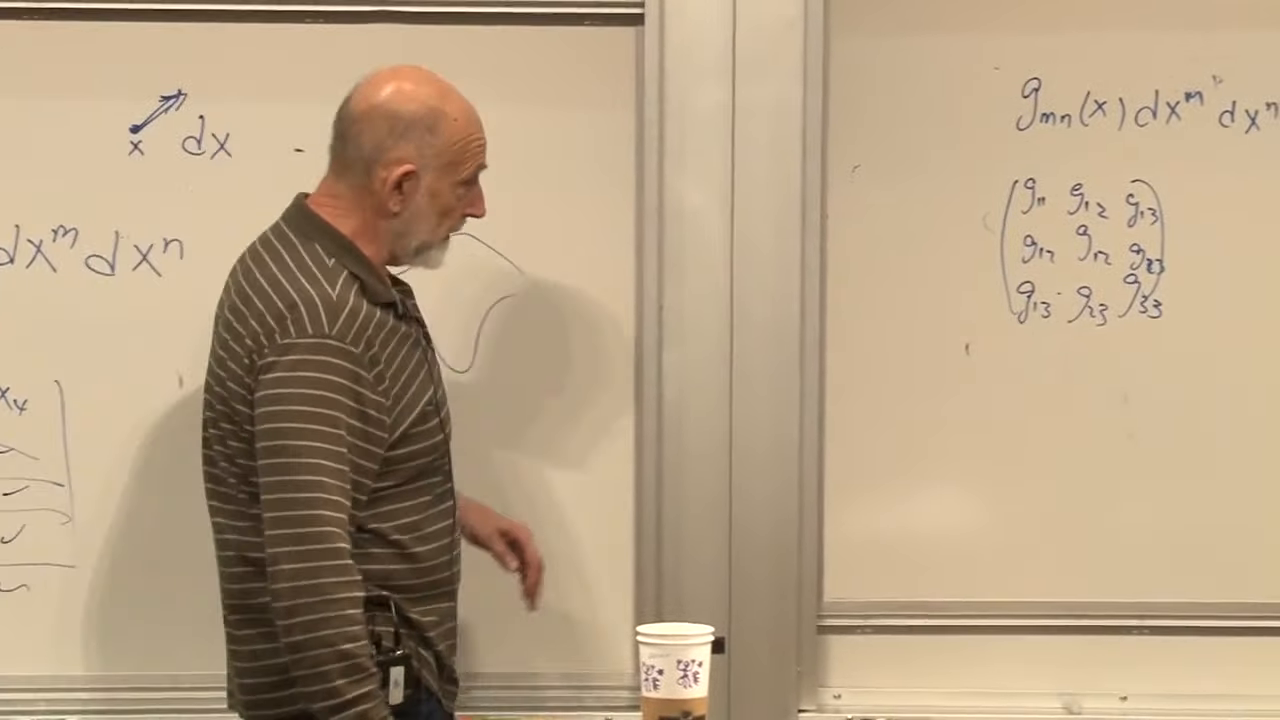
\includegraphics[width=\linewidth]{lecture_02_figure_27.png}
\caption{テンソル変換則が確立された後、対称行列として表示された計量。}
\lectureframe{01:28:50}
\end{figure}

計量は非退化であることが要求される。すなわちゼロ固有値をもたず、したがって逆行列をもつ。その逆行列を\(g^{mn}\)で表す。添字表記では、
\begin{equation}
 g_{mn}g^{np}=\delta_m{}^p.
\label{eq:inverse-metric}
\end{equation}
である。繰り返された\(n\)は和をとられ、\(m\)と\(p\)は積の行と列を表す。

\begin{figure}[H]
\centering
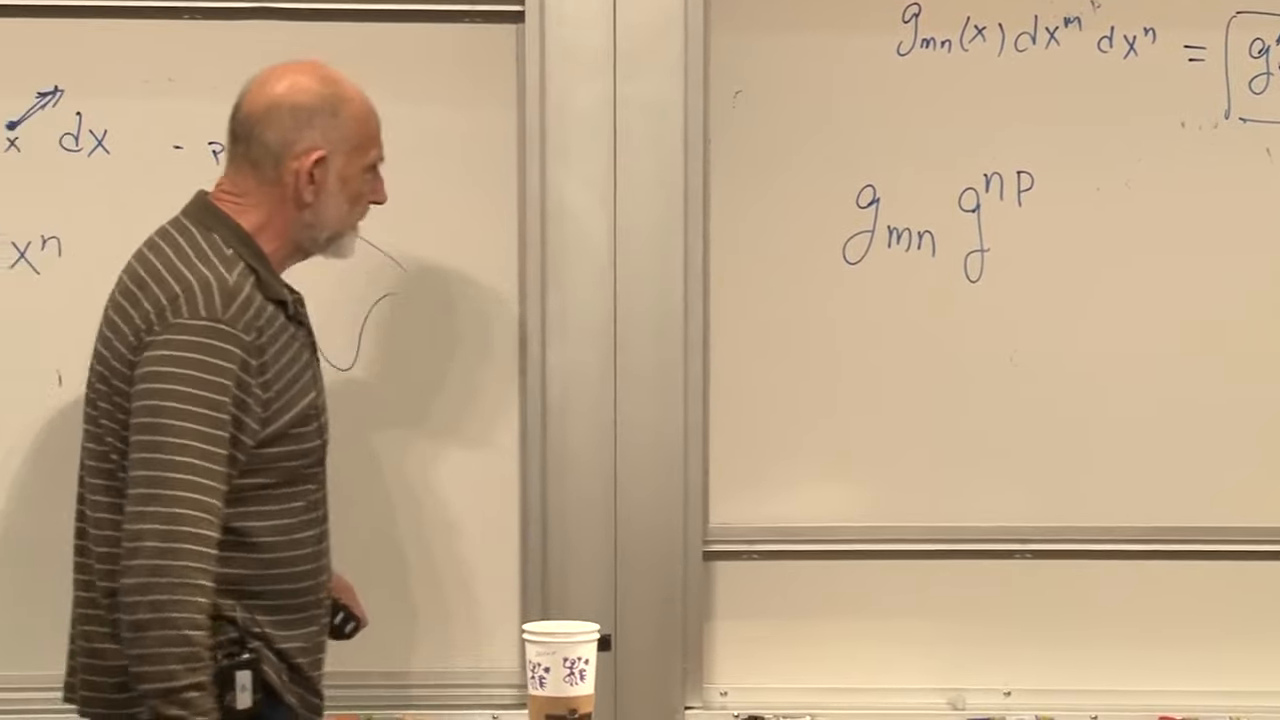
\includegraphics[width=\linewidth]{lecture_02_figure_28.png}
\caption{\(g_{mn}g^{np}=\delta_m{}^p\)を通じて導入される逆計量。}
\lectureframe{01:31:40}
\end{figure}

\begin{classroomqa}
\audiencequestion{ある点におけるベクトルやテンソルは、実際どこに住んでいるのか。}
\lecturerresponse{ある点におけるベクトルはその接空間\(T_P M\)をなし、余ベクトルは双対空間\(T_P^*M\)をなす。より高階のテンソルはこれらの空間のテンソル積に属する。テンソル場は、そのような対象を各点に滑らかに割り当てる。計量は接空間上の双線形形式であり、その逆行列は余接空間上の対応する双線形形式である。\lecturetimestamp{01:34:15}}
\end{classroomqa}

\begin{figure}[H]
\centering
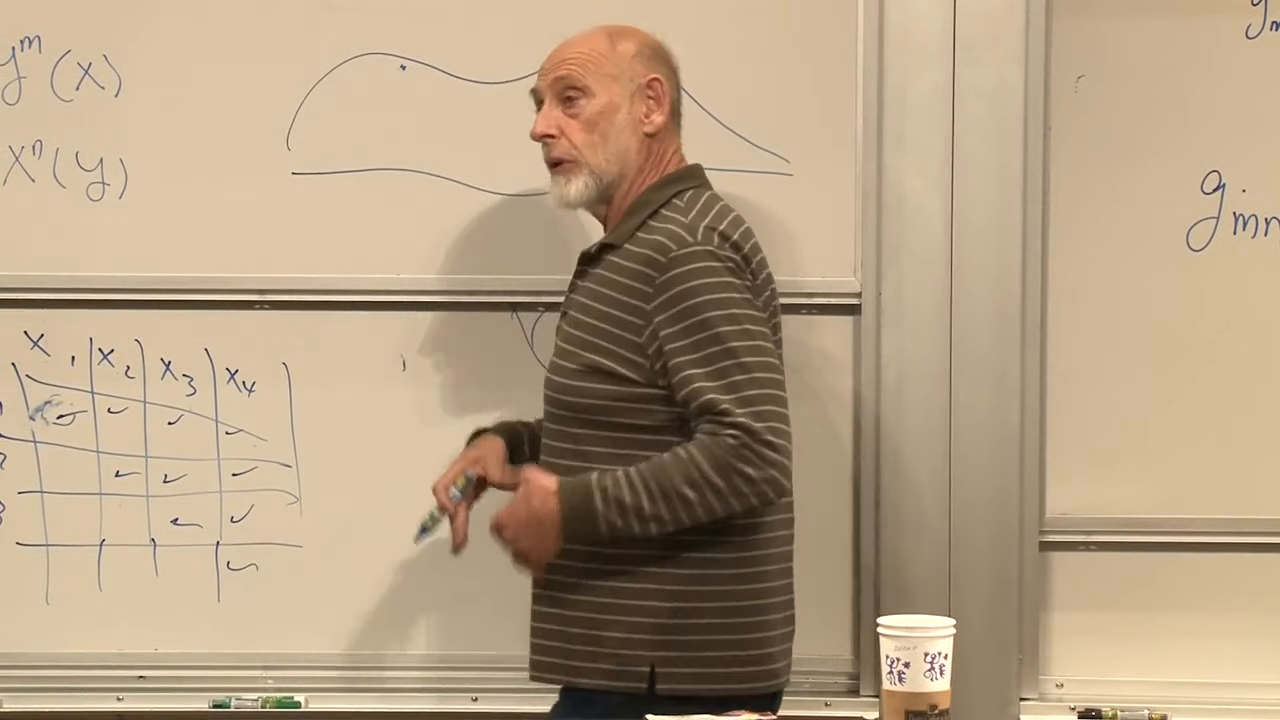
\includegraphics[width=\linewidth]{lecture_02_figure_29.png}
\caption{曲がった多様体の一点に付随する接空間に描かれたベクトル。}
\lectureframe{01:35:45}
\end{figure}

\begin{classroomqa}
\audiencequestion{
\(g_{mn}g^{np}=\delta_m{}^p\)は\(m=p\)の場合のみを指すのか。}
\lecturerresponse{いいえ。それは完全な行列方程式である。各順序対\((m,p)\)に対し、和をとった積は\(m=p\)のとき一であり、\(m\ne p\)のときゼロである。対角および非対角のすべての方程式が同時に含まれている。\lecturetimestamp{01:36:50}}
\end{classroomqa}

\begin{figure}[H]
\centering
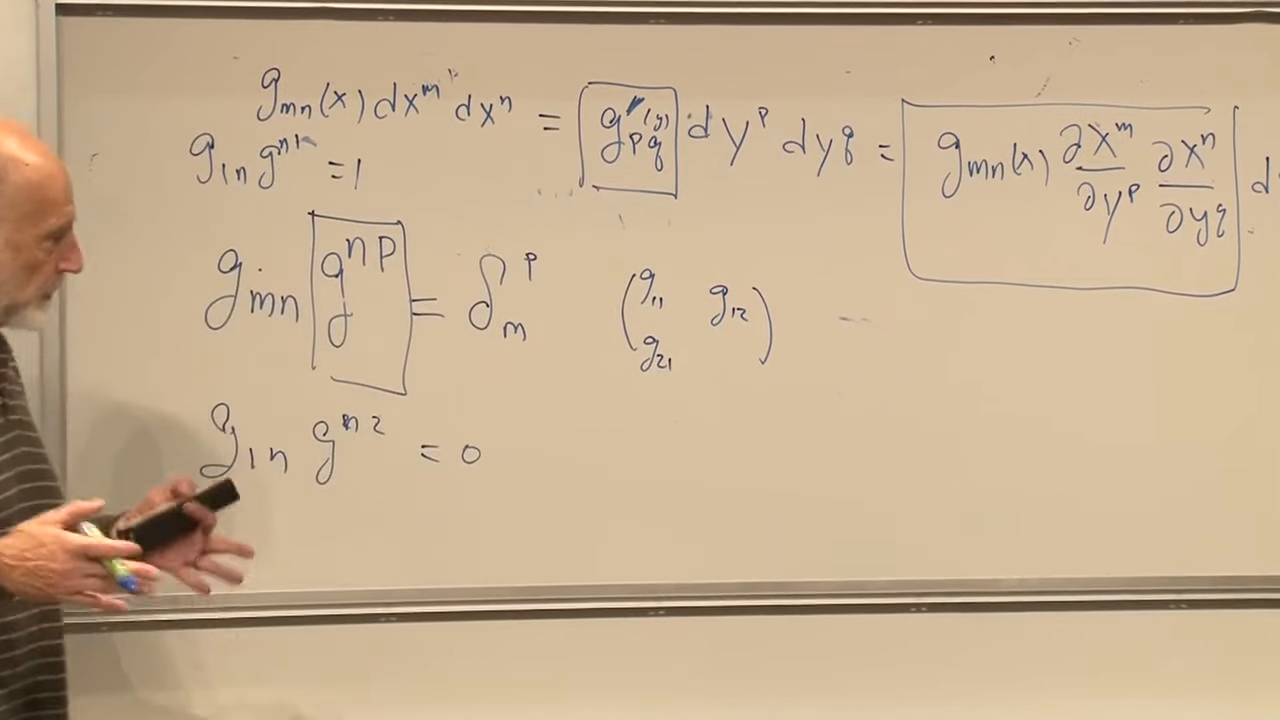
\includegraphics[width=\linewidth]{lecture_02_figure_30.png}
\caption{完全な混合添字の単位行列として解釈された逆関係。}
\lectureframe{01:38:50}
\end{figure}

二次元ではこれは次を意味する。
\begin{equation}
 \begin{pmatrix}
 g_{11} & g_{12}\\
 g_{12} & g_{22}
 \end{pmatrix}
 \begin{pmatrix}
 g^{11} & g^{12}\\
 g^{12} & g^{22}
 \end{pmatrix}
 =
 \begin{pmatrix}
 1&0\\
 0&1
 \end{pmatrix}.
\label{eq:two-dimensional-inverse}
\end{equation}
例えば、
\begin{align}
 g_{11}g^{11}+g_{12}g^{12}&=1,\\
 g_{11}g^{12}+g_{12}g^{22}&=0.
\end{align}
もう一方の行が残りの二つの方程式を与える。

\begin{figure}[H]
\centering
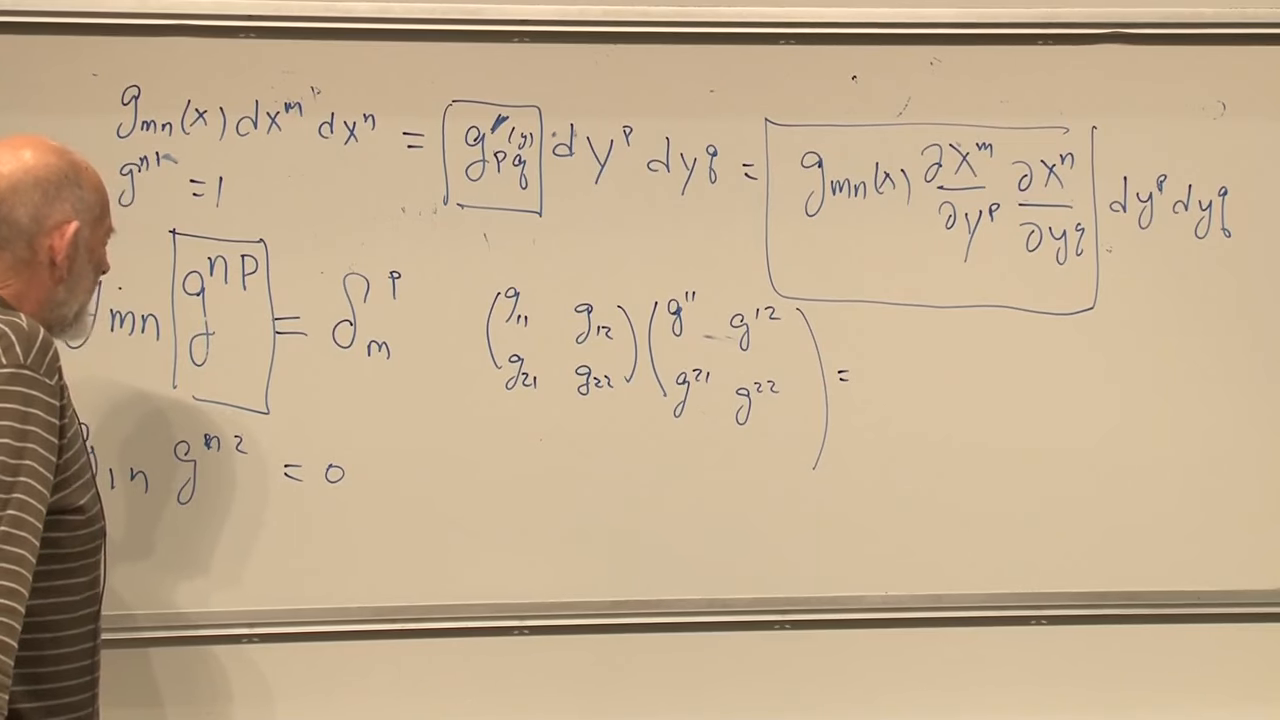
\includegraphics[width=\linewidth]{lecture_02_figure_31.png}
\caption{逆計量の恒等式を、明示的な二次元行列の積として展開したものである。}
\lectureframe{01:40:00}
\end{figure}

\begin{classroomqa}
\audiencequestion{計量は正定値でなければならないのですか。}
\lecturerresponse{通常のリーマン幾何学では、正定値性によって、零でない長さの二乗はすべて正になる。時空は代わりにローレンツ計量を用い、一つの符号が他の三つと逆になっている。ここでどちらの場合にも要求されるのは、正値性ではなく非退化性である。
\lecturetimestamp{01:42:18}}
\end{classroomqa}

\begin{classroomqa}
\audiencequestion{なぜ零固有値を排除するのですか。}
\lecturerresponse{零固有値があると計量行列が特異になり、\(g^{mn}\) は存在せず、計量はベクトルとコベクトルの間に一対一対応を確立できない。通常の微分幾何学的な意味での計量は、非退化であることが要求される。\lecturetimestamp{01:43:56}}
\end{classroomqa}

\begin{classroomqa}
\audiencequestion{四次元計量の十個の独立成分は、十次元弦理論と何か関係があるのですか。}
\lecturerresponse{いいえ。最初の十は単に \(4(4+1)/2\) であり、対称な四行四列行列の成分の数である。超弦理論に十個の時空次元が現れることには、別の起源がある。\lecturetimestamp{01:44:32}}
\end{classroomqa}

\begin{classroomqa}
\audiencequestion{ローレンツ時空に長さが零の零でないベクトルがあると、計量は可逆でなくなるのですか。}
\lecturerresponse{いいえ。零ベクトルは \(g_{mn}V^mV^n=0\) を満たし、不定値二次形式の内部での相殺である。これは \(g_{mn}V^n=0\) を満たす零固有値ベクトルではない。例えば、ミンコフスキー計量は固有値 \(\pm1\) をもち、完全に可逆でありながら、光的ベクトルを許容する。\lecturetimestamp{01:45:02}}
\end{classroomqa}

\section{次に来るもの}

これで幾何学的プログラムを明確に述べることができる。計量は無限小距離を記録し、共変的に変換し、逆をもつ。その成分が複雑に見えるのは、単に座標が複雑だからかもしれない。幾何学自体が曲がっているかどうかを決めるには、隣接する点における計量を座標に依らない方法で比較しなければならない。

通常の微分では十分でない。テンソルを微分すると、その変換則に現れる位置に依存するヤコビアンも微分されるからである。したがって次の段階は共変微分である。計量の微分から接続が構成され、その接続の微分と積から曲率が構成される。そのとき初めて、ページが丸まったという問いは、その最終的な内在的答えを得るのである。
